% =====================================================================
%  ExplicacionKsvd.tex
%  ========================
%
%
%  Descripción:
%  ------------
%  Explicación completa del proyecto 1 de Matemáticas para la
%  Computación, desde cero: de dónde salen los datos, qué es un
%  diccionario, qué es la SVD, cómo funciona OMP y cómo K-SVD junta
%  todo para aprender un diccionario. Cada paso trae un ejemplo
%  resuelto a mano con todas las cuentas y su figura.
%
%
%  Metadata:
%  ----------
%   * Author : zxxz6 (Bryan Violante Arriaga)
%   * Version: 1.0.0
%
%
%  History:
%  ------------
%  Author      Date            Description
%  zxxz6       04/10/2026      Referencias, con la serie SEE Matrix
%  zxxz6       04/10/2026      Derivaciones de los pesos de OMP y del paso SVD
%  zxxz6       03/10/2026      Creation
%
%
% =====================================================================
\documentclass[11pt,letterpaper]{article}

% =====================================================================
%  DATOS DEL DOCUMENTO
% =====================================================================
\newcommand{\materia}{K-SVD desde cero}
\newcommand{\profesor}{Proyecto 1, Matemáticas para la Computación \\
                       Dra. Hayde Peregrina Barreto \\
                       Dr. Luis Villaseñor Pineda}
\newcommand{\periodo}{Otoño 2026}
\newcommand{\alumno}{Bryan Ezequiel Violante Arriaga}

% =====================================================================
%  Preambulo.tex
%  ========================
%
%
%  Descripción:
%  ------------
%  Preámbulo compartido de los apuntes de clase: paquetes, estilo de
%  página, entornos de teorema, las cuatro cajas de color, el estilo de
%  listings y el pseudocódigo en español. Se carga con \input desde
%  cada documento en lugar de copiarlo, para que un arreglo aquí llegue
%  a todas las libretas de una vez.
%
%
%  Considerations:
%  ------------
%  - Se carga con \input y ruta relativa, no con \usepackage, porque
%    \usepackage solo busca en la carpeta del documento y en el árbol
%    de TeX. Un .sty instalado en TEXMFHOME evitaría la ruta, pero vive
%    fuera del repo y una clona nueva no compilaría
%  - Los cuatro datos de la materia se declaran en el documento ANTES
%    del \input. hyperref expande \materia al cargarse, así que si no
%    existe todavía la compilación truena
%  - Cuando la materia la imparte más de un profesor, los nombres van
%    en un solo \profesor separados por \\. La portadilla los imprime
%    dentro de un center, que es donde \\ sí corta renglón. Repetir
%    \newcommand{\profesor} no es opción: truena con "already defined"
%  - algorithmicx no tiene opción de idioma y babel no lo traduce, así
%    que las palabras clave del pseudocódigo se renombran a mano
%  - Los nombres de los entornos van sin acento (\begin{definicion})
%    aunque el rótulo impreso sí lo lleve
%  - babel se carga con es-noshorthands porque en español el " queda
%    activo y se come el texto que le sigue, además de romper listings
%
%
%  Metadata:
%  ----------
%   * Author : zxxz6 (Bryan Violante Arriaga)
%   * Version: 1.7.0
%
%
%  History:
%  ------------
%  Author      Date            Description
%  zxxz6       24/09/2026      Encabezado de una hoja de un ejercicio
%  zxxz6       23/09/2026      Macros de los documentos de soluciones
%  zxxz6       30/08/2026      Macros de lim, limsup y liminf sobre n
%  zxxz6       25/08/2026      Macros de Omega, Theta, o y omega chicas
%  zxxz6       20/08/2026      Cargue pgfplots para graficas de datos
%  zxxz6       20/08/2026      Cargue tikz para diagramas de conjuntos
%  zxxz6       19/08/2026      Documente \profesor con varios nombres
%  zxxz6       19/08/2026      Agregue la caja Idea Random
%  zxxz6       18/08/2026      Creation
%
%
% =====================================================================
%  USO
%  ---
%  \documentclass[11pt,letterpaper]{article}
%  \newcommand{\materia}{...}      % los cuatro datos van arriba
%  \newcommand{\profesor}{...}
%  \newcommand{\periodo}{...}
%  \newcommand{\alumno}{...}
%  \input{../../templates/Preambulo.tex}
%  \begin{document}
%  \portadilla
%
%  Con dos o mas profesores se declara UN solo \profesor y los nombres
%  se separan con \\, uno por renglon:
%
%  \newcommand{\profesor}{Dra. Fulana de Tal \\
%                         Dr. Mengano de Cual}
% =====================================================================


% ==================== IDIOMA Y CODIFICACIÓN ====================
\usepackage[utf8]{inputenc}
\usepackage[T1]{fontenc}
\usepackage[spanish,es-tabla,es-noshorthands]{babel}
\usepackage{lmodern}
\usepackage{microtype}

% ==================== PÁGINA ====================
\usepackage[letterpaper,margin=2.3cm,headheight=14pt]{geometry}
\usepackage{parskip}
\usepackage{fancyhdr}
\usepackage{enumitem}

% ==================== MATEMÁTICAS ====================
\usepackage{amsmath,amssymb,amsthm,mathtools}

% ==================== FIGURAS, TABLAS, CÓDIGO ====================
\usepackage{graphicx}
\usepackage{booktabs}
\usepackage{array}
% float da el especificador [H], que clava una tabla donde se
% escribio. Una traza que LaTeX manda dos paginas adelante deja
% de leerse junto al paso que la produjo
\usepackage{float}
\usepackage{xcolor}
% tikz ya viene arrastrado por tcolorbox[most], pero se carga
% explicito para no depender de ese detalle; la libreria babel
% protege a tikz de los caracteres activos del español
\usepackage{tikz}
\usetikzlibrary{babel}
% pgfplots dibuja graficas de datos (ejes, escalas log) sobre tikz
\usepackage{pgfplots}
\pgfplotsset{compat=1.18}
\usepackage{listings}
\usepackage[ruled,section]{algorithm}
\usepackage{algpseudocode}
\usepackage[most]{tcolorbox}
% soul da \hl, el unico resaltado que parte renglon; \colorbox no
\usepackage{soul}
\usepackage{hyperref}

% =====================================================================
%  ESTILO
% =====================================================================

% --- encabezado y pie de cada página ---
\pagestyle{fancy}
\fancyhf{}
\fancyhead[L]{\small\textsc{\materia}}
\fancyhead[R]{\small\periodo}
\fancyfoot[C]{\small\thepage}
\renewcommand{\headrulewidth}{0.4pt}

% --- enlaces ---
\hypersetup{
  colorlinks=true,
  linkcolor=black,
  urlcolor=blue,
  citecolor=black,
  pdftitle={Apuntes de \materia},
  pdfauthor={\alumno}
}

% --- paleta ---
\definecolor{acento}{HTML}{1F4E79}
\definecolor{fondoIdea}{HTML}{EAF2FB}
\definecolor{fondoOjo}{HTML}{FDF0E6}
\definecolor{fondoPend}{HTML}{F2F0F7}
\definecolor{comentario}{HTML}{5A7D5A}
\definecolor{cadena}{HTML}{A03030}
\definecolor{fondoCodigo}{HTML}{F7F7F7}
\definecolor{fondoResultado}{HTML}{EAF5EC}
\definecolor{marcador}{HTML}{FFF3A3}

% --- entornos de teorema; numeran por sección, o sea por clase ---
\theoremstyle{definition}
\newtheorem{definicion}{Definición}[section]
\newtheorem{ejemplo}[definicion]{Ejemplo}
\newtheorem{ejercicio}[definicion]{Ejercicio}

\theoremstyle{plain}
\newtheorem{teorema}[definicion]{Teorema}
\newtheorem{lema}[definicion]{Lema}
\newtheorem{corolario}[definicion]{Corolario}
\newtheorem{proposicion}[definicion]{Proposición}

\theoremstyle{remark}
\newtheorem*{observacion}{Observación}
\newtheorem*{quick_sum}{Resumen rápido}

% --- cajas de color para lo que se relee antes del examen ---
\newtcolorbox{idea}[1][]{
  colback=fondoIdea, colframe=acento, boxrule=0.6pt,
  arc=2pt, left=6pt, right=6pt, top=5pt, bottom=5pt,
  title={Idea clave}, fonttitle=\bfseries\small, #1
}
\newtcolorbox{ojo}[1][]{
  colback=fondoOjo, colframe=orange!70!black, boxrule=0.6pt,
  arc=2pt, left=6pt, right=6pt, top=5pt, bottom=5pt,
  title={Ojito...}, fonttitle=\bfseries\small, #1
}
\newtcolorbox{pendiente}[1][]{
  colback=fondoPend, colframe=violet!60!black, boxrule=0.6pt,
  arc=2pt, left=6pt, right=6pt, top=5pt, bottom=5pt,
  title={Pendiente por resolver}, fonttitle=\bfseries\small, #1
}
\newtcolorbox{idear}[1][]{
  colback=fondoPend, colframe=pink!60!black, boxrule=0.6pt,
  arc=2pt, left=6pt, right=6pt, top=5pt, bottom=5pt,
  title={Idea Random}, fonttitle=\bfseries\small, #1
}

% --- el resultado al que llego un ejercicio, para que se vea de
%     lejos al hojear la hoja antes del examen ---
\newtcolorbox{resultado}[1][]{
  colback=fondoResultado, colframe=green!45!black, boxrule=0.6pt,
  arc=2pt, left=6pt, right=6pt, top=5pt, bottom=5pt,
  title={Resultado}, fonttitle=\bfseries\small, #1
}

% --- código ---
\lstdefinestyle{codigo}{
  backgroundcolor=\color{fondoCodigo},
  basicstyle=\ttfamily\footnotesize,
  keywordstyle=\color{acento}\bfseries,
  commentstyle=\color{comentario}\itshape,
  stringstyle=\color{cadena},
  numbers=left, numberstyle=\tiny\color{gray}, numbersep=8pt,
  frame=single, rulecolor=\color{gray!40},
  breaklines=true, showstringspaces=false,
  tabsize=4, captionpos=b,
  extendedchars=true, inputencoding=utf8,
  literate={á}{{\'a}}1 {é}{{\'e}}1 {í}{{\'i}}1
           {ó}{{\'o}}1 {ú}{{\'u}}1 {ñ}{{\~n}}1
           {Ü}{{\"U}}1 {ü}{{\"u}}1 {¿}{{?`}}1
           {¡}{{!`}}1
}
\lstset{style=codigo}
\renewcommand{\lstlistingname}{Código}
\renewcommand{\lstlistlistingname}{Índice de código}
% --- pseudocódigo; algorithmicx arma el cuerpo y algorithm el
%     flotante que lo numera y lo pone en el índice. Las palabras
%     clave vienen en inglés de fábrica y babel no las toca, así que
%     se renombran una por una ---
\floatname{algorithm}{Algoritmo}
\renewcommand{\listalgorithmname}{Índice de algoritmos}

\algrenewcommand\algorithmicrequire{\textbf{Entrada:}}
\algrenewcommand\algorithmicensure{\textbf{Salida:}}
\algrenewcommand\algorithmicend{\textbf{fin}}
\algrenewcommand\algorithmicif{\textbf{si}}
\algrenewcommand\algorithmicthen{\textbf{entonces}}
\algrenewcommand\algorithmicelse{\textbf{si no}}
\algrenewcommand\algorithmicfor{\textbf{para}}
\algrenewcommand\algorithmicforall{\textbf{para todo}}
\algrenewcommand\algorithmicdo{\textbf{hacer}}
\algrenewcommand\algorithmicwhile{\textbf{mientras}}
\algrenewcommand\algorithmicrepeat{\textbf{repetir}}
\algrenewcommand\algorithmicuntil{\textbf{hasta que}}
\algrenewcommand\algorithmicloop{\textbf{ciclo}}
\algrenewcommand\algorithmicprocedure{\textbf{procedimiento}}
\algrenewcommand\algorithmicfunction{\textbf{función}}
\algrenewcommand\algorithmicreturn{\textbf{devolver}}
\algrenewcomment[1]{\hfill{\color{comentario}\itshape // #1}}

% Las dos que algorithmicx no trae. El \ del final es obligatorio: sin
% el TeX se come el espacio y sale "hastan-1" en vez de "hasta n-1"
\algnewcommand\Hasta{\textbf{hasta}\ }
\algnewcommand\Intercambiar{\textbf{intercambiar}\ }

% --- abreviaturas que se usan a cada rato ---
\newcommand{\N}{\mathbb{N}}
\newcommand{\Z}{\mathbb{Z}}
\newcommand{\Q}{\mathbb{Q}}
\newcommand{\R}{\mathbb{R}}
\newcommand{\C}{\mathbb{C}}
\newcommand{\abs}[1]{\left\lvert #1 \right\rvert}
\newcommand{\norm}[1]{\left\lVert #1 \right\rVert}
\newcommand{\set}[1]{\left\{ #1 \right\}}
\newcommand{\Ord}[1]{\mathcal{O}\!\left(#1\right)}
% Mayuscula la notacion grande, minuscula la chica
\newcommand{\Omg}[1]{\Omega\!\left(#1\right)}
\newcommand{\Tht}[1]{\Theta\!\left(#1\right)}
\newcommand{\ord}[1]{o\!\left(#1\right)}
\newcommand{\omg}[1]{\omega\!\left(#1\right)}
% Los tres limites sobre n, que salen en cada renglon del criterio
% del cociente para la notacion asintotica
\newcommand{\LM}{\lim_{n \to \infty}}
\newcommand{\LS}{\limsup_{n \to \infty}}
\newcommand{\LI}{\liminf_{n \to \infty}}

% --- encabezado de cada sesión: título a la izquierda, fecha a la
%     derecha. El argumento corto es el que sale en el índice ---
\newcommand{\clase}[2]{%
  \section[#1]{#1 \hfill \normalfont\small\textit{#2}}%
}

% --- portadilla y tabla de contenidos. Se llama una vez, justo
%     despues de \begin{document}. El renglon del profesor va dentro
%     del center, asi que \profesor puede traer varios nombres
%     separados por \\ y salen apilados y centrados sin tocar nada ---
\newcommand{\portadilla}{%
  \begin{center}
    {\LARGE\bfseries\materia\par}
    \vspace{0.4em}
    {\large \profesor \par}
    \vspace{0.2em}
    {\small \periodo\quad-\quad\alumno\par}
    \vspace{0.3em}
    \rule{\linewidth}{0.5pt}
  \end{center}
  \vspace{0.5em}
  \tableofcontents
  \vspace{1em}
  \rule{\linewidth}{0.5pt}%
}

% =====================================================================
%  DOCUMENTOS DE SOLUCIONES
%  Lo que usa una tanda de ejercicios resueltos. Una libreta no toca
%  nada de aqui, pero vive en el preambulo compartido para no tener
%  dos archivos que arreglar cuando cambie el estilo.
% =====================================================================

% --- encabezado compacto: titulo, subtitulo y regla. Sustituye a
%     \portadilla cuando el documento es una tanda de ejercicios: sin
%     indice, porque se hojea de corrido, no se navega ---
\newcommand{\encabezadoSoluciones}[2]{%
  % El paquete algorithm se carga con la opcion [section] para que en
  % una libreta el pseudocodigo se numere por clase. Aqui no hay
  % secciones, asi que esa numeracion sale como "Algoritmo 0.1". Se
  % corrige al vuelo, y solo en los documentos que llaman a este
  % encabezado: la libreta no se entera.
  \renewcommand{\thealgorithm}{\arabic{algorithm}}%
  \begin{center}
    {\LARGE\bfseries #1\par}
    \vspace{0.3em}
    {\small\itshape #2\par}
    \vspace{0.5em}
    \rule{\linewidth}{0.5pt}
  \end{center}
  \vspace{0.3em}%
}

% --- hoja de un solo ejercicio: un renglon chico arriba con el
%     titulo y su numero, y ya. Sin titulo grande y sin pie de pagina,
%     porque en una hoja de dos paginas cada centimetro que se va en
%     adornos es un paso del desarrollo que no cabe ---
\newcommand{\encabezadoEjercicio}[3]{%
  % Misma correccion que en \encabezadoSoluciones: sin secciones, el
  % pseudocodigo saldria numerado "0.1"
  \renewcommand{\thealgorithm}{\arabic{algorithm}}%
  \fancyhf{}%
  \fancyhead[L]{\small\textsc{#1} (ejercicio #2 de #3)}%
  \renewcommand{\headrulewidth}{0.4pt}%
  \pagestyle{fancy}%
  \thispagestyle{fancy}%
}

% --- bloque tematico, numerado con romanos: I, II, III. Agrupa los
%     ejercicios que comparten tema. No dibuja regla: la del
%     \problema que sigue ya separa el titulo del primer ejercicio,
%     y dos rayas seguidas dejan un hueco feo ---
\newcounter{parte}
\renewcommand{\theparte}{\Roman{parte}}
\newcommand{\parte}[1]{%
  \bigskip
  \refstepcounter{parte}%
  \noindent{\large\bfseries \theparte. #1\par}%
}

% --- un ejercicio resuelto. Se numera solo y corrido a lo largo del
%     documento, sin reiniciar en cada parte, para poder decir "el 14"
%     sin aclarar de que bloque ---
\newcounter{problema}
\newcommand{\problema}[1]{%
  \bigskip
  \noindent\rule{\linewidth}{0.4pt}\par
  \vspace{0.3em}
  \refstepcounter{problema}%
  \noindent{\bfseries Ejercicio \theproblema\ --- #1\par}
  \vspace{0.3em}%
}

% --- rotulo del paso que sigue: Caso base, Hipotesis inductiva, Paso
%     inductivo. El texto sigue en el mismo renglon ---
\newcommand{\paso}[1]{\par\vspace{0.3em}\noindent\textbf{#1}\ }

% --- la respuesta de un ejercicio, centrada y en un cuadro. El
%     argumento va en modo matematico, sin los delimitadores ---
\newcommand{\respuesta}[1]{%
  \[
    \boxed{\;#1\;}
  \]
}

% --- resaltado inline, como pasarle el plumon a media frase. No
%     admite matematicas adentro: soul rompe con $...$, asi que una
%     formula que hay que destacar va en \respuesta ---
\sethlcolor{marcador}
\newcommand{\resaltar}[1]{\hl{#1}}

% --- justificacion al final de un renglon de \align, en chiquito y
%     entre parentesis, para decir de donde salio el paso ---
\newcommand{\razon}[1]{\quad\text{\small\itshape (#1)}}

%############################ END OF PREAMBULO.TEX #############################
%###############################################################################


\usetikzlibrary{positioning,arrows.meta,decorations.pathreplacing,
                calc,fit}
\graphicspath{{img/}}

% --- un color por átomo del ejemplo, los mismos de las figuras ---
\definecolor{atomoA}{HTML}{2A78D6}
\definecolor{atomoB}{HTML}{EB6834}
\definecolor{atomoC}{HTML}{1BAF7A}
\definecolor{atomoE}{HTML}{C98500}
\definecolor{tinta}{HTML}{52514E}

\newcommand{\cA}[1]{\textcolor{atomoA}{#1}}
\newcommand{\cB}[1]{\textcolor{atomoB}{#1}}
\newcommand{\cC}[1]{\textcolor{atomoC}{#1}}
\newcommand{\cE}[1]{\textcolor{atomoE}{#1}}

% --- notación que se repite ---
\newcommand{\T}{^{\mathsf{T}}}
\newcommand{\raiz}[1]{\sqrt{#1}}

% =====================================================================
\begin{document}
% =====================================================================

\portadilla
\newpage

% =====================================================================
%  1. Introducción
% =====================================================================

\section{Introducción: qué es K-SVD y para qué sirve}

\begin{quick_sum}
    Este documento explica el proyecto completo sin suponer que se sabe
    nada de antemano. Primero repasa las herramientas de álgebra lineal
    que se usan; después sigue los datos desde el ECG hasta la matriz
    $X$, explica qué es un diccionario, qué es la SVD, cómo funciona OMP
    y cómo K-SVD junta todo. Cada concepto trae un ejemplo chico
    resuelto a mano con todas las cuentas.
\end{quick_sum}

\subsection*{El objetivo del proyecto}

El enunciado pide implementar K-SVD y obtener una \textbf{base
entrenada} para algún tipo de señal, de manera que se pueda comparar la
señal original con su reconstrucción hecha a partir de una
representación dispersa.

Dicho más simple: se quiere aprender, a partir de un electrocardiograma
(ECG), un conjunto de \textbf{formas básicas}, y después demostrar que
cualquier pedazo de ese ECG se puede volver a armar sumando \textbf{muy
pocas} de esas formas.

\subsection*{La idea central: armar cosas con pocas piezas}

Piensa en un juego de piezas de construcción. Con un juego de 256
piezas distintas se arman muchísimas figuras, y cada figura usa solo
unas cuantas piezas, no las 256. Si las piezas son buenas, cualquier
figura sale con pocas; si son malas, cada figura necesita muchas o no
sale bien.

En el proyecto la correspondencia es esta:

\begin{center}
\begin{tabular}{lll}
    \toprule
    \textbf{Juego de piezas} & \textbf{Proyecto} & \textbf{Tamaño} \\
    \midrule
    una pieza          & un \textbf{átomo}: una forma de onda
                       & 128 números \\
    el juego completo  & el \textbf{diccionario} $D$
                       & 256 átomos \\
    una figura         & una \textbf{ventana}: un pedazo del ECG
                       & 128 números \\
    las instrucciones  & los \textbf{pesos} $\alpha$
                       & casi todos en cero \\
    \bottomrule
\end{tabular}
\end{center}

K-SVD es el algoritmo que \textbf{aprende buenas piezas}: empieza con
piezas más o menos al azar y las va mejorando hasta que con pocas se
arma cualquier pedazo del ECG.

\subsection*{Por qué importa que sean pocas}

A esto se le llama \textbf{representación dispersa}: dispersa porque
casi todos los pesos valen cero. Sirve para tres cosas.

\begin{itemize}[itemsep=0.3em]
    \item \textbf{Comprimir.} Una ventana son 128 números. Si se arma
          con 8 átomos, basta guardar 8 índices y 8 pesos.
    \item \textbf{Quitar ruido.} El ruido no se parece a ningún átomo,
          así que al reconstruir con pocos átomos se queda fuera.
    \item \textbf{Entender la señal.} Los átomos aprendidos son las
          formas que más se repiten. En el ECG resultan ser los picos
          del latido y sus ondas.
\end{itemize}

\subsection*{El algoritmo en una mirada}

K-SVD repite dos pasos. En cada uno se deja algo fijo y se mejora lo
otro. La figura~\ref{fig:ciclo} lo resume; cada caja tiene su sección
más adelante.

\begin{figure}[H]
\centering
\begin{tikzpicture}[
    caja/.style={draw=tinta, rounded corners=3pt, fill=fondoIdea,
                 align=center, font=\small, minimum height=1.1cm,
                 text width=4.6cm},
    flecha/.style={-{Stealth[length=2.5mm]}, thick, tinta},
    node distance=0.9cm and 1.4cm]
    \node[caja] (x) {Ventanas del ECG\\$X$, de $128 \times 2539$};
    \node[caja, right=of x] (d0)
        {Diccionario inicial $D_0$\\256 ventanas al azar};
    \node[caja, below=of d0, fill=atomoA!15] (omp)
        {\textbf{Paso 1: OMP}\\$D$ fijo; cada ventana escoge\\
         pocos átomos $\to \alpha$};
    \node[caja, below=of omp, fill=atomoB!15] (svd)
        {\textbf{Paso 2: SVD}\\cada átomo se ajusta a las\\
         ventanas que lo usan $\to D$};
    \node[caja, left=of svd] (fin)
        {Diccionario entrenado\\formas típicas del latido};
    \draw[flecha] (x) -- (d0);
    \draw[flecha] (d0) -- (omp);
    \draw[flecha] (omp) -- (svd);
    \draw[flecha] (svd.east) -- ++(0.8,0) |- (omp.east)
        node[pos=0.25, right, font=\small, align=left]
        {repetir\\20 veces};
    \draw[flecha] (svd) -- (fin);
\end{tikzpicture}
\caption{El ciclo de K-SVD.}
\label{fig:ciclo}
\end{figure}

Se parece a \textbf{k-means}, el algoritmo de agrupamiento. En k-means
cada punto usa exactamente un centroide, y actualizar un centroide es
sacar un promedio. En K-SVD cada ventana usa varios átomos, y
actualizar un átomo es sacar una SVD. El nombre sale de ahí: $K$
átomos, cada uno actualizado con una \textbf{SVD}.

\subsection*{El ejemplo de juguete}

Casi todo se explica con un ejemplo que cabe en una hoja: átomos de 3
números en lugar de 128, y 4 átomos en lugar de 256. Los números se
escogieron a mano para que las cuentas salgan limpias.

\[
    D =
    \begin{pmatrix}
        \cA{1} & \cB{0.6} & \cC{0} & \cE{0} \\
        \cA{0} & \cB{0.8} & \cC{0} & \cE{1} \\
        \cA{0} & \cB{0}   & \cC{1} & \cE{0}
    \end{pmatrix}
    \qquad
    X =
    \begin{pmatrix}
        1   & 0.9 \\
        1   & 1   \\
        0.5 & 0
    \end{pmatrix}
\]

Las columnas de $D$ son los átomos \cA{$A$}, \cB{$B$}, \cC{$C$} y
\cE{$E$}; las de $X$ son dos ventanas, $v_1$ y $v_2$. El proyecto real
funciona exactamente igual, solo que más grande:

\begin{center}
\begin{tabular}{lcc}
    \toprule
                            & \textbf{Juguete} & \textbf{Proyecto} \\
    \midrule
    largo de una ventana    & 3            & 128 muestras \\
    número de átomos        & 4            & 256 \\
    número de ventanas      & 2            & 2539 de entrenamiento \\
    tamaño de $D$           & $3 \times 4$ & $128 \times 256$ \\
    tamaño de $X$           & $3 \times 2$ & $128 \times 2539$ \\
    \bottomrule
\end{tabular}
\end{center}

\newpage

% =====================================================================
%  2. Herramientas
% =====================================================================

\section{Las herramientas de álgebra lineal}

\begin{quick_sum}
    Todo K-SVD se escribe con unas pocas operaciones: vectores,
    producto punto, norma, matrices, matriz por vector, la matriz de
    rango 1 y los eigenvalores. Aquí se repasan una por una, cada una
    con un ejemplo, y diciendo para qué se va a usar.
\end{quick_sum}

\subsection*{Vectores}

\begin{definicion}[Vector]
    Un \textbf{vector} es una lista ordenada de números. Cada número es
    una \textbf{componente}. En este documento los vectores se escriben
    de pie, como columna:
    \[
        v = \begin{pmatrix} 1 \\ 1 \\ 0.5 \end{pmatrix}
        \qquad \text{o, para ahorrar espacio,} \qquad
        v = (1,\ 1,\ 0.5).
    \]
\end{definicion}

Una ventana del ECG es un vector de 128 componentes; un átomo, también.

Dos operaciones básicas se hacen componente por componente:

\begin{ejemplo}[Suma y multiplicación por un número]
    \begin{align*}
        0.25 \cdot (1,\ 0,\ 0)
            &= (0.25,\ 0,\ 0) \\
        1.25 \cdot (0.6,\ 0.8,\ 0)
            &= (1.25 \cdot 0.6,\ 1.25 \cdot 0.8,\ 1.25 \cdot 0)
             = (0.75,\ 1,\ 0) \\
        (0.25,\ 0,\ 0) + (0.75,\ 1,\ 0)
            &= (0.25 + 0.75,\ 0 + 1,\ 0 + 0) = (1,\ 1,\ 0)
    \end{align*}
\end{ejemplo}

Sumar vectores multiplicados por números se llama hacer una
\textbf{combinación lineal}. Es exactamente lo que se hace al armar una
ventana con átomos: cada átomo por su peso, y todo sumado.

\subsection*{Producto punto}

\begin{definicion}[Producto punto]
    El \textbf{producto punto} de dos vectores del mismo tamaño
    multiplica componente por componente y suma todo:
    \[
        u \cdot v = u_1 v_1 + u_2 v_2 + \cdots + u_n v_n .
    \]
    El resultado es un solo número.
\end{definicion}

\begin{ejemplo}
    Con $B = (0.6,\ 0.8,\ 0)$ y $x = (1,\ 1,\ 0.5)$:
    \[
        B \cdot x = (0.6)(1) + (0.8)(1) + (0)(0.5)
                  = 0.6 + 0.8 + 0 = 1.4 .
    \]
\end{ejemplo}

\begin{idea}
    El producto punto mide \textbf{qué tanto se parecen} dos vectores.
    Si los dos miden 1, el producto punto es el coseno del ángulo entre
    ellos:
    \begin{itemize}[itemsep=0.1em]
        \item vale $1$ si apuntan exactamente igual;
        \item vale $0$ si son perpendiculares, es decir, si no tienen
              nada en común;
        \item vale $-1$ si apuntan exactamente al revés.
    \end{itemize}
    OMP usa esto para decidir qué átomo se parece más a lo que falta
    por explicar de una ventana.
\end{idea}

\subsection*{Norma: el largo de un vector}

\begin{definicion}[Norma]
    La \textbf{norma} de un vector es su largo: la raíz de la suma de
    los cuadrados de sus componentes,
    \[
        \norm{v} = \raiz{v_1^2 + v_2^2 + \cdots + v_n^2}
                 = \raiz{v \cdot v} .
    \]
\end{definicion}

\begin{ejemplo}
    \[
        \norm{(1,\ 1,\ 0.5)} = \raiz{1^2 + 1^2 + 0.5^2}
                             = \raiz{1 + 1 + 0.25}
                             = \raiz{2.25} = 1.5 .
    \]
\end{ejemplo}

Un vector de norma 1 se llama \textbf{unitario}. Cualquier vector
distinto de cero se vuelve unitario dividiéndolo entre su norma; a eso
se le llama \textbf{normalizar}:
\[
    \frac{(1,\ 1,\ 0.5)}{1.5} = (0.667,\ 0.667,\ 0.333),
    \qquad
    \norm{(0.667,\ 0.667,\ 0.333)} = 1 .
\]
Normalizar conserva la dirección y solo cambia el largo. Todos los
átomos del diccionario son unitarios.

\subsection*{Vectores perpendiculares}

Dos vectores son \textbf{perpendiculares} (u \textbf{ortogonales}) si su
producto punto es cero. Con los átomos del ejemplo:
\begin{align*}
    A \cdot E &= (1)(0) + (0)(1) + (0)(0) = 0
        && \text{perpendiculares} \\
    A \cdot B &= (1)(0.6) + (0)(0.8) + (0)(0) = 0.6
        && \text{no perpendiculares}
\end{align*}

\begin{ojo}
    En un espacio de $n$ dimensiones caben como máximo $n$ vectores
    perpendiculares entre sí: en 3 dimensiones, 3 (los tres ejes). El
    ejemplo tiene 4 átomos en 3 dimensiones, así que forzosamente
    algunos no son perpendiculares. En el proyecto pasa lo mismo: 256
    átomos en 128 dimensiones.
\end{ojo}

\subsection*{Matrices}

Una \textbf{matriz} es una tabla de números. Una matriz de
$m \times n$ tiene $m$ filas y $n$ columnas. Se puede leer como $n$
vectores columna puestos uno al lado del otro: así se leen $D$ (una
columna por átomo) y $X$ (una columna por ventana).

La \textbf{transpuesta} $M\T$ convierte filas en columnas:
\[
    M = \begin{pmatrix} 1 & 0 \\ 0 & 1 \\ 1 & 1 \end{pmatrix}
    \quad\Longrightarrow\quad
    M\T = \begin{pmatrix} 1 & 0 & 1 \\ 0 & 1 & 1 \end{pmatrix} .
\]
Una matriz es \textbf{simétrica} si es igual a su transpuesta.

\subsection*{Matriz por vector: dos maneras de leerlo}

Multiplicar una matriz por un vector tiene dos lecturas, y las dos se
usan en el proyecto.

\begin{ejemplo}[Fila por fila]
    Cada componente del resultado es el producto punto de una fila de
    la matriz con el vector:
    \[
        \begin{pmatrix} 1 & 2 \\ 0 & 1 \\ 3 & 0 \end{pmatrix}
        \begin{pmatrix} 2 \\ 1 \end{pmatrix}
        =
        \begin{pmatrix}
            1 \cdot 2 + 2 \cdot 1 \\
            0 \cdot 2 + 1 \cdot 1 \\
            3 \cdot 2 + 0 \cdot 1
        \end{pmatrix}
        =
        \begin{pmatrix} 4 \\ 1 \\ 6 \end{pmatrix} .
    \]
\end{ejemplo}

\begin{ejemplo}[Como combinación de columnas]
    El mismo producto es la suma de las columnas de la matriz, cada
    una multiplicada por la componente correspondiente del vector:
    \[
        \begin{pmatrix}
            \cA{1} & \cB{2} \\ \cA{0} & \cB{1} \\ \cA{3} & \cB{0}
        \end{pmatrix}
        \begin{pmatrix} \cA{2} \\ \cB{1} \end{pmatrix}
        = \cA{2} \begin{pmatrix} \cA{1} \\ \cA{0} \\ \cA{3}
                 \end{pmatrix}
        + \cB{1} \begin{pmatrix} \cB{2} \\ \cB{1} \\ \cB{0}
                 \end{pmatrix}
        = \begin{pmatrix} 4 \\ 1 \\ 6 \end{pmatrix} .
    \]
\end{ejemplo}

\begin{idea}
    La segunda lectura es la clave de todo el proyecto:
    \[
        D\,\alpha = \alpha_1 d_1 + \alpha_2 d_2 + \cdots
                  + \alpha_{256}\, d_{256} .
    \]
    Multiplicar el diccionario por el vector de pesos \emph{es} armar
    la ventana sumando átomos. Si casi todos los $\alpha_i$ son cero,
    la ventana se arma con pocos átomos.
\end{idea}

\subsection*{Matriz por matriz}

Para multiplicar $M$ por $N$ se multiplica $M$ por cada columna de $N$,
y los resultados se ponen como columnas. La entrada $(i,j)$ del
resultado es el producto punto de la fila $i$ de $M$ con la columna $j$
de $N$. Para que se pueda, el número de columnas de $M$ debe ser igual
al número de filas de $N$:
\[
    (m \times k) \cdot (k \times n) = m \times n
    \qquad \text{(las dos } k \text{ deben coincidir).}
\]

Un caso que aparece mucho es $M\T M$. Su entrada $(i,j)$ es el
producto punto de la columna $i$ de $M$ con la columna $j$ de $M$:
\[
    M\T M =
    \begin{pmatrix} 1 & 0 & 1 \\ 0 & 1 & 1 \end{pmatrix}
    \begin{pmatrix} 1 & 0 \\ 0 & 1 \\ 1 & 1 \end{pmatrix}
    =
    \begin{pmatrix}
        1\cdot1 + 0\cdot0 + 1\cdot1 & 1\cdot0 + 0\cdot1 + 1\cdot1 \\
        0\cdot1 + 1\cdot0 + 1\cdot1 & 0\cdot0 + 1\cdot1 + 1\cdot1
    \end{pmatrix}
    =
    \begin{pmatrix} 2 & 1 \\ 1 & 2 \end{pmatrix} .
\]
$M\T M$ siempre es cuadrada y simétrica. La SVD la usa.

\subsection*{Columna por fila: matrices de rango 1}

Una columna de $m$ números por una fila de $n$ números da una matriz de
$m \times n$. Cada columna del resultado es la misma columna original,
multiplicada por un número distinto:
\[
    \begin{pmatrix} \cA{1} \\ \cA{2} \\ \cA{0} \end{pmatrix}
    \begin{pmatrix} 3 & 1 \end{pmatrix}
    =
    \begin{pmatrix}
        3 \cdot \cA{1} & 1 \cdot \cA{1} \\
        3 \cdot \cA{2} & 1 \cdot \cA{2} \\
        3 \cdot \cA{0} & 1 \cdot \cA{0}
    \end{pmatrix}
    =
    \begin{pmatrix} 3 & 1 \\ 6 & 2 \\ 0 & 0 \end{pmatrix} .
\]

\begin{definicion}[Matriz de rango 1]
    Una matriz es de \textbf{rango 1} si se puede escribir como una
    columna por una fila. Todas sus columnas apuntan en la misma
    dirección; solo cambian de tamaño.
\end{definicion}

\begin{idea}
    Un átomo (una columna) por sus pesos en varias ventanas (una fila)
    es una matriz de rango 1. Por eso, al actualizar un átomo, K-SVD
    busca la mejor aproximación de rango 1 de una matriz, y eso lo da
    la SVD.
\end{idea}

\subsection*{Matrices ortogonales}

\begin{definicion}[Matriz ortogonal]
    Una matriz cuadrada $Q$ es \textbf{ortogonal} si $Q\T Q = I$. Es
    lo mismo que decir que sus columnas miden 1 y son perpendiculares
    entre sí, porque la entrada $(i,j)$ de $Q\T Q$ es el producto punto
    de la columna $i$ con la columna $j$.
\end{definicion}

Una matriz ortogonal es una \textbf{rotación} (o un reflejo): no
cambia largos ni ángulos. Su inversa es gratis, porque es su
transpuesta. Por ejemplo, girar un cuarto de vuelta:
\[
    Q = \begin{pmatrix} 0 & -1 \\ 1 & 0 \end{pmatrix},
    \qquad
    Q\T Q =
    \begin{pmatrix} 0 & 1 \\ -1 & 0 \end{pmatrix}
    \begin{pmatrix} 0 & -1 \\ 1 & 0 \end{pmatrix}
    = \begin{pmatrix} 1 & 0 \\ 0 & 1 \end{pmatrix} .
\]

\begin{ojo}
    Simétrica y ortogonal son cosas distintas. La matriz
    $\left(\begin{smallmatrix} 2 & 1 \\ 1 & 2 \end{smallmatrix}\right)$
    es simétrica pero no ortogonal: su primera columna, $(2, 1)$, mide
    $\raiz{5}$ y no 1. No gira, estira.
\end{ojo}

\subsection*{Sistemas de ecuaciones con infinitas soluciones}

Una ecuación con dos incógnitas, como $x + y = 2$, tiene infinitas
soluciones: $(1, 1)$, $(2, 0)$, $(0, 2)$, $(1.5, 0.5)$\ldots{} Si se
pide la solución \textbf{con más ceros}, quedan dos: $(2, 0)$ y
$(0, 2)$.

\begin{idea}
    Es justo la situación del proyecto. Cada ventana da 128 ecuaciones
    ($x = D\alpha$, una por muestra) y hay 256 incógnitas (un peso por
    átomo). Hay infinitas soluciones, y de todas se busca la que tiene
    más ceros. Eso es lo que hace OMP.
\end{idea}

\subsection*{Eigenvalores y eigenvectores}

\begin{definicion}[Eigenvalor y eigenvector]
    Un vector $v \neq 0$ es \textbf{eigenvector} de una matriz cuadrada
    $M$ si $M v = \lambda v$ para algún número $\lambda$, su
    \textbf{eigenvalor}. Es una dirección que $M$ no gira: solo la
    estira o la encoge por $\lambda$.
\end{definicion}

Los eigenvalores son las raíces de $\det(M - \lambda I) = 0$. Para una
matriz de $2 \times 2$ el determinante es
$\det\left(\begin{smallmatrix} a & b \\ c & d
\end{smallmatrix}\right) = ad - bc$.

\begin{ejemplo}
    Con $M = \left(\begin{smallmatrix} 2 & 1 \\ 1 & 2
    \end{smallmatrix}\right)$:
    \begin{align*}
        \det(M - \lambda I)
            &= \det\begin{pmatrix} 2 - \lambda & 1 \\
                                   1 & 2 - \lambda \end{pmatrix}
             = (2 - \lambda)^2 - 1 \\
            &= \lambda^2 - 4\lambda + 3
             = (\lambda - 3)(\lambda - 1) = 0 .
    \end{align*}
    Los eigenvalores son $\lambda_1 = 3$ y $\lambda_2 = 1$. Para cada
    uno se resuelve $(M - \lambda I) v = 0$:
    \begin{align*}
        \lambda_1 = 3: &\quad
        \begin{pmatrix} -1 & 1 \\ 1 & -1 \end{pmatrix} v = 0
        \;\Rightarrow\; v = (1,\ 1) , \\
        \lambda_2 = 1: &\quad
        \begin{pmatrix} 1 & 1 \\ 1 & 1 \end{pmatrix} v = 0
        \;\Rightarrow\; v = (1,\ -1) .
    \end{align*}
    Comprobación: $M (1, 1) = (2 + 1,\ 1 + 2) = (3, 3) = 3\,(1, 1)$.
\end{ejemplo}

\begin{idea}
    En el ejemplo, $(1, 1) \cdot (1, -1) = 0$: los dos eigenvectores
    son perpendiculares. No es casualidad. El \textbf{teorema
    espectral} dice que los eigenvectores de una matriz simétrica
    siempre se pueden escoger perpendiculares entre sí. Gracias a eso
    la SVD siempre tiene rotaciones.
\end{idea}

\newpage

% =====================================================================
%  3. Datos
% =====================================================================

\section{Los datos: del ECG a la matriz $X$}

\begin{quick_sum}
    El ECG llega como una tira de 650\,000 números. Se corta en 5078
    pedazos de 128, se pone cada pedazo como columna de una matriz, y a
    cada columna se le quita su promedio y se normaliza. El resultado
    es $X$, la matriz con la que trabaja K-SVD.
\end{quick_sum}

\subsection*{La señal}

Un electrocardiograma mide el voltaje eléctrico del corazón a lo largo
del tiempo. Se usa el \textbf{registro 100} de la base \textbf{MIT-BIH
Arrhythmia}, de PhysioNet: 30 minutos del ECG de un paciente real.

El aparato mide el voltaje \textbf{360 veces por segundo}. Cada
medición es un número en milivolts (mV) y se llama \textbf{muestra}.
La lista completa de muestras, en orden de tiempo, es la
\textbf{señal}:
\begin{align*}
    \text{senal}[0]      &= -0.145 \text{ mV}
        && \text{el voltaje en } t = 0.000 \text{ s} \\
    \text{senal}[1]      &= -0.145 \text{ mV}
        && \text{el voltaje en } t = 0.003 \text{ s} \\
    &\;\;\vdots \\
    \text{senal}[649999] &= -1.280 \text{ mV}
        && \text{el voltaje en } t = 1805.6 \text{ s}
\end{align*}
Son $650\,000 / 360 = 1805.6$ segundos, o sea 30.1 minutos. En numpy es
un arreglo de \textbf{una sola dimensión}, de forma \texttt{(650000,)}.
El archivo original trae dos canales, uno por cada par de electrodos;
\texttt{cargar\_ecg()} se queda solo con el primero.

\begin{figure}[H]
\centering
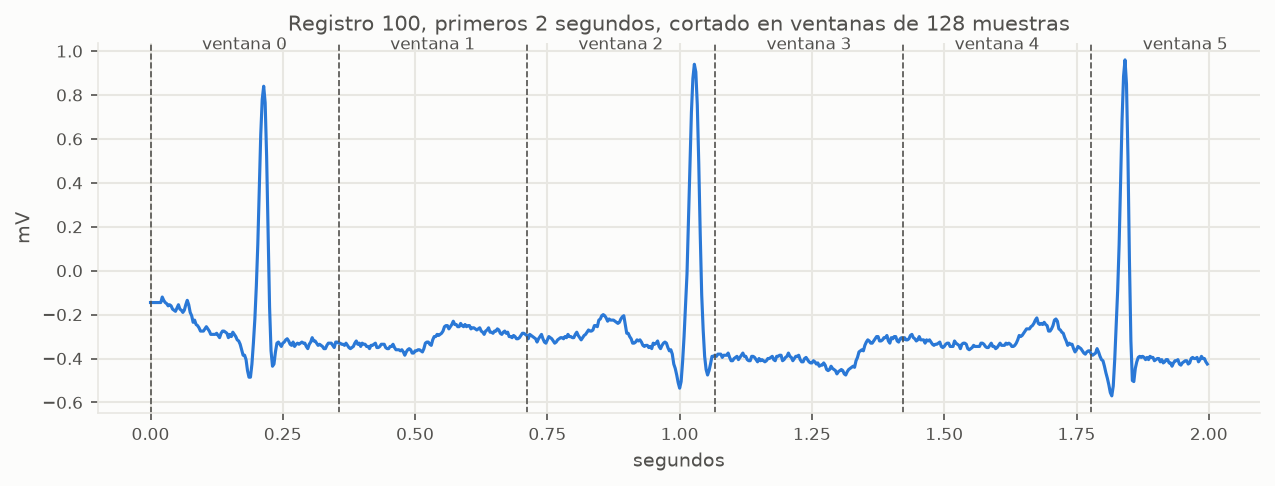
\includegraphics[width=\linewidth]{ecg_ventanas.png}
\caption{Los primeros dos segundos de la señal. Cada pico alto es un
latido (el complejo QRS). Las líneas punteadas son los cortes de las
ventanas de la siguiente sección.}
\label{fig:ecg}
\end{figure}

\subsection*{Las ventanas}

K-SVD no recibe la señal entera. La señal se \textbf{corta en pedazos
del mismo tamaño}, uno tras otro, y a cada pedazo se le llama
\textbf{ventana}. Cada ventana se pone \textbf{de pie, como columna}, y
las columnas se acomodan una al lado de la otra. La
figura~\ref{fig:ventanas} lo muestra con una señal de 12 muestras y
ventanas de 4.

\begin{figure}[H]
\centering
\begin{tikzpicture}[
    x=8mm, y=7mm,
    celda/.style={draw=tinta, minimum width=7.5mm, minimum height=6.5mm,
                  inner sep=0pt, font=\small},
    llave/.style={decorate, decoration={brace, mirror, amplitude=4pt},
                  thick, tinta}]
    \node[font=\small, anchor=east] at (-0.7, 0) {señal};
    \foreach \v [count=\i from 0] in {5,6,7,8}
        \node[celda, fill=atomoA!20] at (\i, 0) {\v};
    \foreach \v [count=\i from 4] in {1,2,3,4}
        \node[celda, fill=atomoB!20] at (\i, 0) {\v};
    \foreach \v [count=\i from 8] in {9,9,0,0}
        \node[celda, fill=atomoC!20] at (\i, 0) {\v};
    \draw[llave] (-0.45, -0.6) -- (3.45, -0.6)
        node[midway, below=5pt, font=\small] {ventana 0};
    \draw[llave] (3.55, -0.6) -- (7.45, -0.6)
        node[midway, below=5pt, font=\small] {ventana 1};
    \draw[llave] (7.55, -0.6) -- (11.45, -0.6)
        node[midway, below=5pt, font=\small] {ventana 2};

    \foreach \v [count=\r from 0] in {5,6,7,8}
        \node[celda, fill=atomoA!20] at (4.5, -3.2 - \r) {\v};
    \foreach \v [count=\r from 0] in {1,2,3,4}
        \node[celda, fill=atomoB!20] at (5.5, -3.2 - \r) {\v};
    \foreach \v [count=\r from 0] in {9,9,0,0}
        \node[celda, fill=atomoC!20] at (6.5, -3.2 - \r) {\v};
    \foreach \k in {0,1,2}
        \node[font=\scriptsize] at (4.5 + \k, -2.45) {v\k};
    \foreach \r in {0,1,2,3}
        \node[font=\scriptsize, anchor=east] at (3.9, -3.2 - \r)
            {muestra \r};
    \draw[-{Stealth[length=2.5mm]}, thick, tinta]
        (5.5, -1.75) -- (5.5, -2.3);
    \node[font=\small, anchor=west] at (7.2, -4.7)
        {matriz de $4 \times 3$};
\end{tikzpicture}
\caption{Una señal de 12 muestras cortada en ventanas de 4. Cada
ventana pasa a ser una columna.}
\label{fig:ventanas}
\end{figure}

Hay tres palabras que no hay que confundir:
\begin{itemize}[itemsep=0.2em]
    \item \textbf{señal}: todo el arreglo (650\,000 números);
    \item \textbf{muestra}: un solo número de la señal;
    \item \textbf{ventana}: un pedazo de muestras seguidas (128).
\end{itemize}

\subsubsection*{En el proyecto}

Las ventanas son de 128 muestras (\texttt{TAM\_VENTANA = 128} en
\texttt{Utils.py}):
\[
    \frac{650\,000}{128} = 5078.1
    \;\Rightarrow\; 5078 \text{ ventanas completas},
    \qquad
    650\,000 - 5078 \cdot 128 = 16 \text{ muestras que sobran.}
\]
Las 16 que sobran no alcanzan para una ventana y se descartan. No se
rellenan con ceros, porque eso inventaría una forma de onda que no
existe en el ECG. La ventana $j$ es la columna
\[
    \text{ventana } j = \text{senal}[128j \;:\; 128j + 128],
\]
que cubre de $0.356\,j$ a $0.356\,(j+1)$ segundos. La matriz de ventanas
crudas mide $128 \times 5078$; su esquina superior izquierda es
\[
    \begin{array}{r|rrrrrr}
        & \text{v}0 & \text{v}1 & \text{v}2 & \text{v}3 & \text{v}4
        & \text{v}5 \\
        \hline
        \text{muestra } 0 & -0.145 & -0.330 & -0.295 & -0.385
                          & -0.315 & -0.380 \\
        \text{muestra } 1 & -0.145 & -0.330 & -0.310 & -0.390
                          & -0.305 & -0.385 \\
        \text{muestra } 2 & -0.145 & -0.335 & -0.290 & -0.380
                          & -0.315 & -0.380 \\
        \vdots & & & & & & \vdots
    \end{array}
\]
Casi todo vale alrededor de $-0.3$ mV: es la \textbf{línea base}, donde
el corazón no hace nada visible. En la ventana 5, alrededor de la fila
23, sí hay un latido:
\[
    \begin{array}{c|ccccccccc}
        \text{fila} & 19 & 20 & 21 & 22 & \mathbf{23} & 24 & 25 & 26
                    & 27 \\
        \hline
        \text{mV} & 0.120 & 0.410 & 0.690 & 0.885 & \mathbf{0.960}
                  & 0.850 & 0.520 & 0.050 & -0.320
    \end{array}
\]

\subsubsection*{Por qué se corta en ventanas}

\begin{enumerate}[itemsep=0.3em]
    \item \textbf{K-SVD aprende de lo que se repite entre muchos
          ejemplos.} La señal entera es un solo ejemplo; cortada, da
          5078. El corazón repite casi la misma forma en cada latido,
          así que muchas ventanas se parecen, y eso es justo lo que el
          diccionario aprende.
    \item \textbf{Los átomos miden lo mismo que una ventana}, porque se
          suman para reconstruirla. Con la señal entera, cada átomo
          sería un ECG de 30 minutos, y habría que aprender 256 de ellos
          a partir de un solo ejemplo.
    \item \textbf{Costo.} OMP y la SVD trabajan con matrices del tamaño
          de una ventana. Con 128 filas las cuentas son chicas.
\end{enumerate}

\subsubsection*{Por qué 128}

Una ventana de 128 muestras dura $128 / 360 = 0.356$ segundos. Un
complejo QRS dura unos 100 ms, así que cabe completo y con margen. Un
latido completo dura unos 800 ms y no cabe. Es lo bastante largo para
que quepa la forma importante del latido y lo bastante corto para tener
muchos ejemplos. Que sea potencia de 2 es costumbre, no necesidad: OMP
y K-SVD funcionan igual con 120 o con 150.

\subsubsection*{Por qué cada ventana es una columna}

Porque en álgebra lineal un vector se escribe como columna, y así se
escribe toda la teoría del proyecto:
\[
    \underbrace{x}_{128 \times 1}
    = \underbrace{D}_{128 \times 256}\;
      \underbrace{\alpha}_{256 \times 1}
    \qquad\qquad
    \underbrace{X}_{128 \times 5078}
    = \underbrace{D}_{128 \times 256}\;
      \underbrace{\alpha}_{256 \times 5078} .
\]
Con las ventanas como columnas, una sola multiplicación reconstruye
todas a la vez. Como filas también funcionaría, pero todo quedaría
transpuesto y el código dejaría de leerse como las fórmulas.

\subsection*{Centrar y normalizar}

Antes de entrar a $X$, a cada ventana (cada columna) se le hacen dos
cosas:
\[
    \text{1. centrar: } c \leftarrow c - \operatorname{promedio}(c),
    \qquad
    \text{2. normalizar: } c \leftarrow \frac{c}{\norm{c}} .
\]
El objetivo es que dos ventanas con \textbf{la misma forma} queden
\textbf{iguales}, aunque el ECG las haya medido más arriba, más abajo,
más fuertes o más débiles. Al diccionario solo le interesa la forma.

\begin{ejemplo}[Centrar quita la altura]
    Dos ventanas con la misma forma, pero una medida 5 unidades más
    arriba porque la línea base subió con la respiración:
    \begin{align*}
        P &= (0,\ 0,\ 4,\ 0), & \operatorname{promedio}(P)
            &= (0 + 0 + 4 + 0)/4 = 1, \\
        Q &= (5,\ 5,\ 9,\ 5), & \operatorname{promedio}(Q)
            &= (5 + 5 + 9 + 5)/4 = 6 .
    \end{align*}
    Restando a cada una su promedio:
    \[
        P - 1 = (-1,\ -1,\ 3,\ -1), \qquad
        Q - 6 = (-1,\ -1,\ 3,\ -1) .
    \]
    Quedan iguales. Sin centrar, el diccionario gastaría átomos en
    aprender ``qué tan arriba está la línea'', que no es parte del
    latido; el primer átomo aprendido sería una línea plana.
\end{ejemplo}

\begin{ejemplo}[Normalizar quita el tamaño]
    Dos ventanas con la misma forma, una el doble de fuerte:
    \begin{align*}
        P &= (-1,\ -1,\ 3,\ -1), &
        \norm{P} &= \raiz{1 + 1 + 9 + 1} = \raiz{12} = 3.464, \\
        R &= (-2,\ -2,\ 6,\ -2), &
        \norm{R} &= \raiz{4 + 4 + 36 + 4} = \raiz{48} = 6.928 .
    \end{align*}
    Dividiendo cada una entre su norma:
    \[
        \frac{P}{3.464} = \frac{R}{6.928}
        = (-0.289,\ -0.289,\ 0.866,\ -0.289) .
    \]
    Otra vez iguales, y ahora miden exactamente 1.
\end{ejemplo}

\begin{ojo}
    Sin normalizar, K-SVD le haría más caso a las ventanas grandes,
    porque pesan más en el error. Y OMP compara con productos punto,
    que crecen con el tamaño: una ventana grande se vería ``más
    parecida'' a todo solo por ser grande.
\end{ojo}

\begin{ejemplo}[Con los números reales]
    La ventana 5 tiene su pico de 0.960 mV en la fila 23. Su promedio
    es $-0.3494$, y ya centrada su norma es $2.8586$. Entonces el valor
    que queda en $X$ es
    \[
        \frac{0.960 - (-0.3494)}{2.8586}
        = \frac{1.3094}{2.8586} = 0.458 .
    \]
\end{ejemplo}

\begin{figure}[H]
\centering
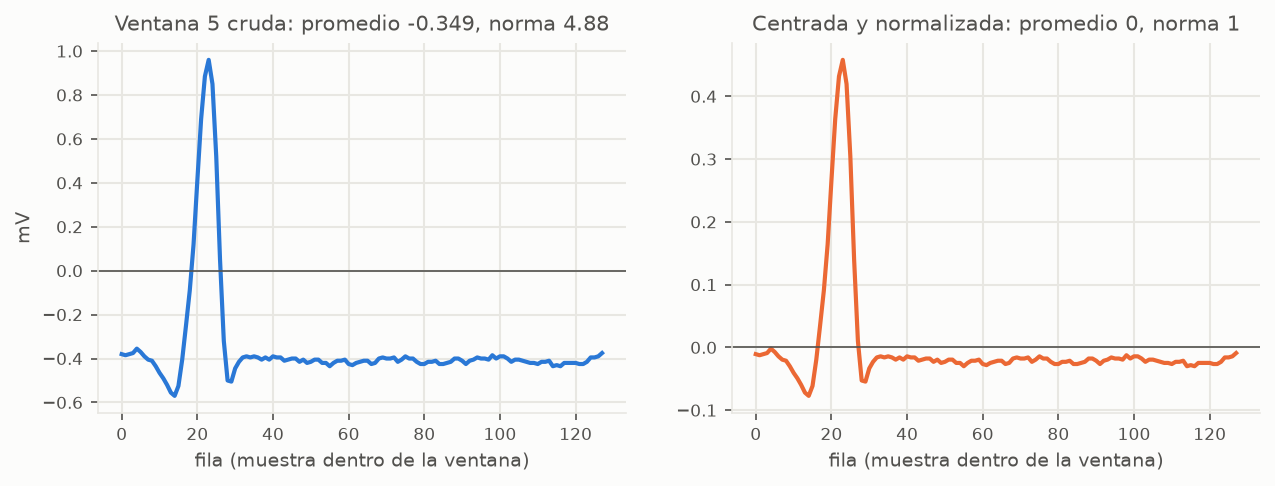
\includegraphics[width=\linewidth]{ventana_normalizada.png}
\caption{La ventana 5 antes y después de centrar y normalizar. Los
números cambian pero la forma no: el pico sigue en la fila 23.}
\end{figure}

\subsection*{La matriz $X$}

$X$ tiene la misma forma que las ventanas crudas, $128 \times 5078$,
pero cada columna tiene promedio 0 y norma 1. Vista como mapa de
calor (figura~\ref{fig:x}), cada franja vertical es una ventana; las
manchas rojas son los picos de los latidos, y caen en filas distintas
porque los latidos no quedan en la misma posición dentro de cada
ventana. Esa variación es lo que el diccionario tiene que aprender a
cubrir.

\begin{figure}[H]
\centering
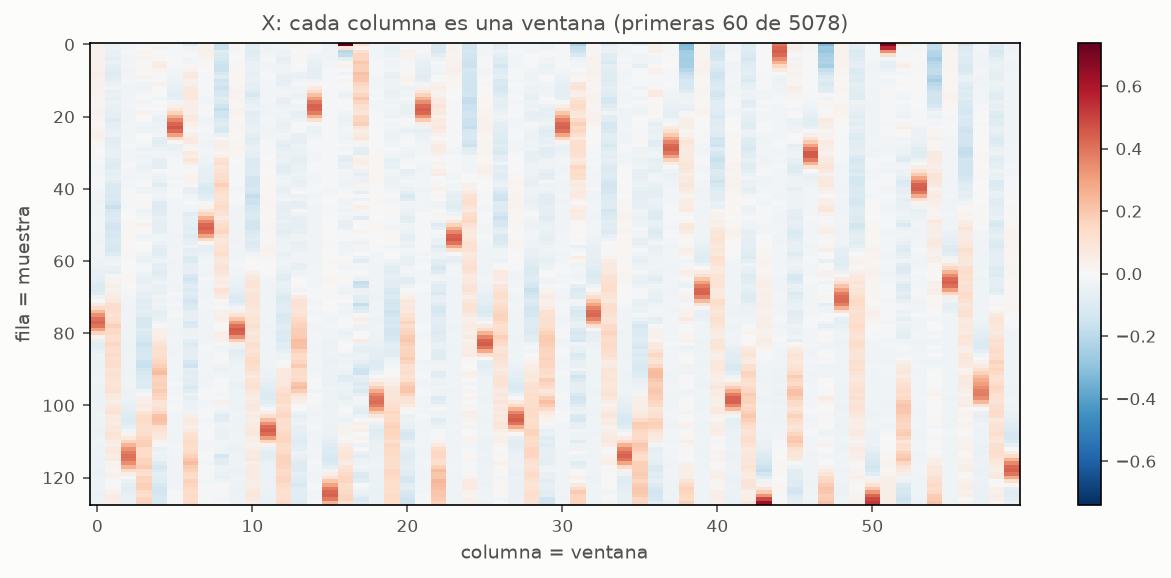
\includegraphics[width=0.92\linewidth]{matriz_x.png}
\caption{Las primeras 60 columnas de $X$.}
\label{fig:x}
\end{figure}

\subsection*{Entrenamiento y prueba}

$X$ se parte a la mitad \textbf{en orden de tiempo}: las primeras 2539
ventanas entrenan y las últimas 2539 se usan al final para medir. No se
reparte al azar porque las ventanas contiguas de un ECG se parecen
muchísimo; al azar, en la prueba quedarían vecinas directas de las de
entrenamiento, y el resultado se vería mejor de lo que es.

\subsection*{Varios pacientes}

Con \texttt{Experimento.py -{}-todos} se cargan los 48 registros de
MIT-BIH. Cada paciente se corta en ventanas \textbf{por separado} y
después se pegan las columnas, hasta $128 \times 243\,744$. Si primero
se pegaran las señales y luego se cortara, alguna ventana quedaría con
la mitad de un paciente y la mitad de otro: una forma que no existe. La
partición entrenamiento y prueba también se hace dentro de cada
paciente.

\newpage

% =====================================================================
%  4. Diccionario
% =====================================================================

\section{El diccionario: átomos, $D$ y $\alpha$}

\begin{quick_sum}
    Un átomo es una forma de onda del tamaño de una ventana. El
    diccionario $D$ los junta como columnas. Los pesos $\alpha$ dicen
    cuánto de cada átomo usa cada ventana, y $D\alpha$ reconstruye las
    ventanas. Aquí se presenta el ejemplo de juguete que usan las
    secciones de OMP y de actualización de átomos.
\end{quick_sum}

\subsection*{Qué es un átomo y qué es el diccionario}

\begin{definicion}[Átomo]
    Un \textbf{átomo} es un vector del mismo tamaño que una ventana,
    con norma 1. Por sí solo no es un pedazo real del ECG: es una pieza
    con la que se arman pedazos.
\end{definicion}

Que mida 1 importa: así el átomo solo aporta \textbf{forma}, y el
tamaño lo pone su peso. Si los átomos tuvieran largos distintos, al
compararlos con una ventana ganarían los más largos por ser largos, no
por parecerse más.

\begin{definicion}[Diccionario]
    El \textbf{diccionario} $D$ es la matriz cuyas columnas son todos
    los átomos:
    \[
        D = \begin{pmatrix}
                | & | & & | \\
                d_0 & d_1 & \cdots & d_{255} \\
                | & | & & |
            \end{pmatrix},
        \qquad 128 \times 256 .
    \]
\end{definicion}

Las \textbf{columnas} de $D$ son los átomos. Las \textbf{filas} son la
posición en el tiempo dentro del átomo: la fila 23 de $D$ es el mismo
instante que la fila 23 de una ventana. Por eso, al sumar átomos, cada
instante cae justo en su instante de la ventana.

Se llama diccionario por la analogía con uno de palabras: con un
vocabulario fijo se escriben muchísimas oraciones, y cada oración usa
pocas palabras. Aquí el vocabulario son formas de onda y las oraciones
son ventanas.

\subsection*{El ejemplo de juguete}

\begin{center}
\begin{tabular}{cc}
    \toprule
    \textbf{Átomos} & \textbf{Ventanas} \\
    \midrule
    \cA{$A = (1,\ 0,\ 0)$}     & $v_1 = (1,\ 1,\ 0.5)$ \\
    \cB{$B = (0.6,\ 0.8,\ 0)$} & $v_2 = (0.9,\ 1,\ 0)$ \\
    \cC{$C = (0,\ 0,\ 1)$}     & \\
    \cE{$E = (0,\ 1,\ 0)$}     & \\
    \bottomrule
\end{tabular}
\end{center}

Todos los átomos miden 1; por ejemplo,
$\norm{B} = \raiz{0.6^2 + 0.8^2} = \raiz{0.36 + 0.64} = 1$.

\begin{figure}[H]
\centering
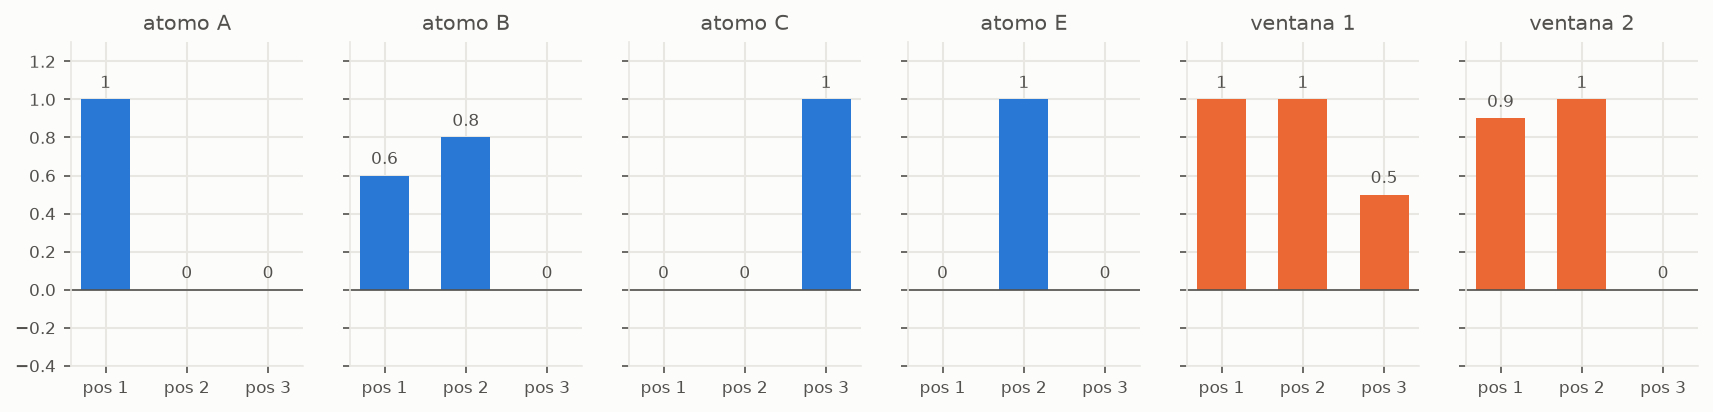
\includegraphics[width=\linewidth]{atomos_juguete.png}
\caption{Los cuatro átomos y las dos ventanas del ejemplo, una barra
por componente.}
\end{figure}

\subsection*{$\alpha$: los pesos}

Para cada ventana, $\alpha$ es un \textbf{vector} con un peso por
átomo. Cada entrada es un número que dice cuánto de ese átomo se usa;
un cero quiere decir que el átomo no se usa. Para la ventana 1:
\[
    \alpha^{(1)} = \bigl(\, \cA{0.25},\ \cB{1.25},\ \cC{0.5},\ \cE{0}
                   \,\bigr) .
\]
De dónde salen estos números se desarrolla cuenta por cuenta en la
sección de OMP; por ahora basta saber que los calcula OMP.

\subsubsection*{Reconstruir una ventana}

La ventana se arma sumando cada átomo por su peso. Es la lectura de
matriz por vector como combinación de columnas:
\[
    D\,\alpha^{(1)} =
    \begin{pmatrix}
        \cA{1} & \cB{0.6} & \cC{0} & \cE{0} \\
        \cA{0} & \cB{0.8} & \cC{0} & \cE{1} \\
        \cA{0} & \cB{0}   & \cC{1} & \cE{0}
    \end{pmatrix}
    \begin{pmatrix} \cA{0.25} \\ \cB{1.25} \\ \cC{0.5} \\ \cE{0}
    \end{pmatrix}
    = \cA{0.25} \begin{pmatrix} \cA{1} \\ \cA{0} \\ \cA{0}
                \end{pmatrix}
    + \cB{1.25} \begin{pmatrix} \cB{0.6} \\ \cB{0.8} \\ \cB{0}
                \end{pmatrix}
    + \cC{0.5} \begin{pmatrix} \cC{0} \\ \cC{0} \\ \cC{1}
                \end{pmatrix} .
\]
Haciendo cada multiplicación y sumando:
\[
    \begin{pmatrix} 0.25 \\ 0 \\ 0 \end{pmatrix}
    + \begin{pmatrix} 0.75 \\ 1 \\ 0 \end{pmatrix}
    + \begin{pmatrix} 0 \\ 0 \\ 0.5 \end{pmatrix}
    = \begin{pmatrix} 1 \\ 1 \\ 0.5 \end{pmatrix} = v_1 .
\]
La ventana 1 sale exacta con tres átomos.

\subsubsection*{$\alpha$ de todas las ventanas: una matriz}

Cada ventana tiene su vector de pesos. Puestos como columnas, $\alpha$
es una \textbf{matriz} con una fila por átomo y una columna por
ventana:
\[
    \alpha =
    \begin{pmatrix}
        0.25 & 0    \\
        1.25 & 1.34 \\
        0.5  & 0    \\
        0    & 0
    \end{pmatrix}
    \begin{matrix} \leftarrow \cA{A} \\ \leftarrow \cB{B} \\
                   \leftarrow \cC{C} \\ \leftarrow \cE{E}
    \end{matrix}
    \qquad
    \text{columnas: } v_1,\ v_2 .
\]
Se lee de dos maneras:
\begin{itemize}[itemsep=0.3em]
    \item \textbf{por columna}: la receta de una ventana. La ventana 2
          es $1.34 \cdot B$;
    \item \textbf{por fila}: qué ventanas usan un átomo. La fila $B$
          tiene dos números distintos de cero, así que $B$ lo usan las
          dos ventanas. Esta lectura es la que usa la actualización de
          átomos.
\end{itemize}

Una sola multiplicación reconstruye todo:
\[
    D\,\alpha =
    \begin{pmatrix} 1 & 0.804 \\ 1 & 1.072 \\ 0.5 & 0 \end{pmatrix}
    \qquad \text{contra} \qquad
    X =
    \begin{pmatrix} 1 & 0.9 \\ 1 & 1 \\ 0.5 & 0 \end{pmatrix} .
\]
La ventana 1 sale exacta; la ventana 2 no, le falta
$(0.096,\ -0.072,\ 0)$. OMP se detuvo ahí porque el error ya era menor
que el objetivo, como se verá.

\subsubsection*{En el proyecto: casi todo es cero}

En el proyecto $\alpha$ mide $256 \times 2539$, y en cada columna solo
unas 8 a 11 entradas son distintas de cero. La figura~\ref{fig:disperso}
ilustra cómo se ve una matriz así.

\begin{figure}[H]
\centering
\begin{tikzpicture}[x=4.5mm, y=4.5mm]
    \fill[fondoPend] (0, 0) rectangle (16, -12);
    \foreach \c/\f in {0/2, 0/7, 1/5, 1/9, 1/11, 2/0, 2/7, 3/3, 3/10,
                       4/2, 4/8, 4/11, 5/1, 5/6, 6/4, 6/9, 7/0, 7/7,
                       7/10, 8/3, 8/5, 9/2, 9/8, 10/6, 10/11, 11/1,
                       11/4, 11/9, 12/0, 12/7, 13/5, 13/10, 14/3,
                       14/8, 14/11, 15/2, 15/6}
        \fill[atomoA] (\c, -\f) rectangle (\c + 1, -\f - 1);
    \draw[step=1, white, line width=0.8pt] (0, 0) grid (16, -12);
    \draw[tinta] (0, 0) rectangle (16, -12);
    \node[font=\small, above] at (8, 0) {ventanas (columnas)};
    \node[font=\small, rotate=90, above] at (0, -6)
        {átomos (filas)};
    \node[font=\small, anchor=west, align=left] at (16.6, -6)
        {azul: peso distinto de cero\\gris: peso cero};
\end{tikzpicture}
\caption{Ilustración de una matriz $\alpha$ dispersa: cada ventana usa
solo unos pocos átomos.}
\label{fig:disperso}
\end{figure}

\subsection*{Por qué 256 átomos}

Tiene que haber \textbf{más átomos que muestras por ventana}. Con 128
átomos independientes, cada ventana se arma de una sola manera, y casi
siempre con muchos átomos. Con 256 se puede armar de muchas maneras, y
se escoge la que usa menos. Un diccionario con más átomos que
dimensiones se llama \textbf{sobrecompleto}: el sistema $x = D\alpha$
queda con 128 ecuaciones y 256 incógnitas, con infinitas soluciones.

No se usan muchos más porque con 2539 ventanas de entrenamiento y 256
átomos, cada átomo se ajusta con unas 10 ventanas en promedio; con 1000
átomos serían 2 o 3, muy pocas. Además algunos quedarían sin uso, y el
entrenamiento tarda en proporción al número de átomos. En la literatura
se usan de 2 a 4 veces más átomos que el tamaño de la señal.

\subsection*{Los átomos no son perpendiculares}

Con 256 átomos en 128 dimensiones, forzosamente muchos se ``pisan''. En
el ejemplo, $A \cdot B = 0.6$. Medido en el diccionario inicial real:

\begin{center}
\begin{tabular}{lc}
    \toprule
    \textbf{$|$coseno$|$ entre átomos distintos} & \textbf{Valor} \\
    \midrule
    máximo (dos casi iguales)            & 0.995 \\
    promedio                             & 0.226 \\
    pares casi perpendiculares ($< 0.1$) & 35\,\% \\
    \bottomrule
\end{tabular}
\end{center}

\begin{ojo}
    Es una diferencia importante con la SVD, donde $U$ y $V$ sí son
    ortogonales. Y tiene una consecuencia en OMP: como los átomos se
    pisan, los pesos no se pueden sacar con un producto punto cada uno;
    hay que resolver un sistema. Se ve en la vuelta 3 del ejemplo de
    OMP.
\end{ojo}

\subsection*{El diccionario inicial y cuándo cambia}

Al empezar, los 256 átomos son \textbf{256 ventanas reales de $X$
escogidas al azar}, normalizadas. Así el entrenamiento arranca con
formas que ya parecen de ECG y no con ruido.

\begin{figure}[H]
\centering
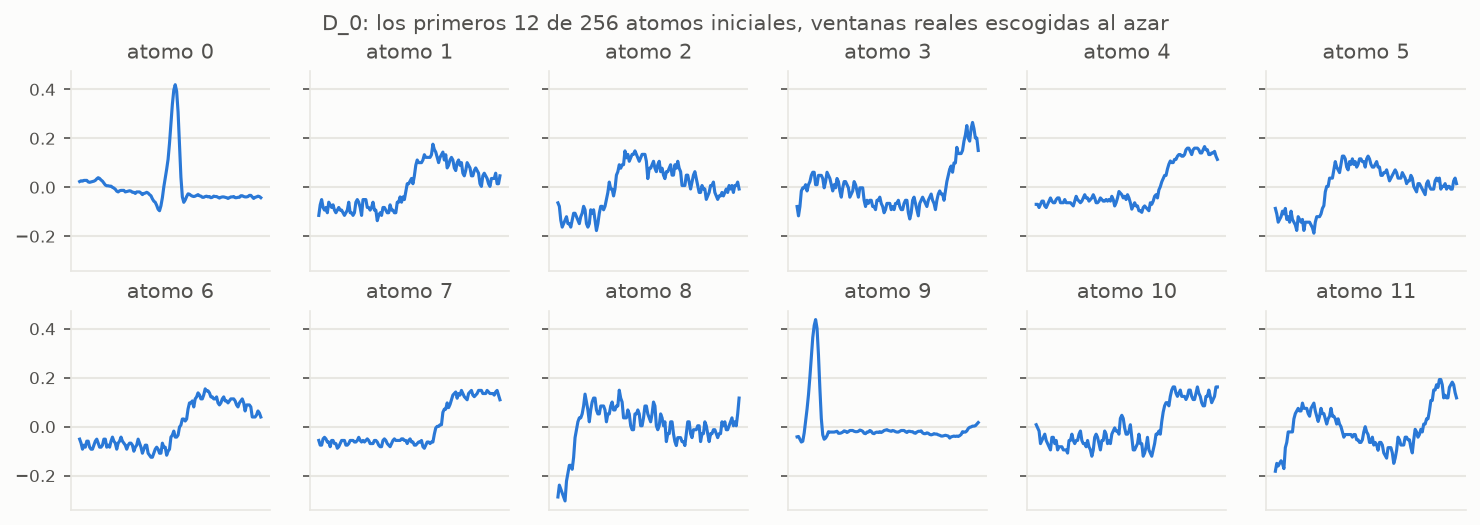
\includegraphics[width=\linewidth]{diccionario_inicial.png}
\caption{Doce de los 256 átomos iniciales. Algunos tienen un pico y
otros solo un escalón de la línea base.}
\end{figure}

El diccionario cambia \textbf{solo durante el entrenamiento}, y solo en
el paso 2 de cada iteración. En el paso 1, OMP lo usa sin modificarlo.
Al terminar las 20 iteraciones queda fijo, se guarda en
\texttt{out/modelo.npz} y se usa tal cual para reconstruir las ventanas
de prueba.

\newpage

% =====================================================================
%  5. SVD
% =====================================================================

\section{La SVD: descomposición en valores singulares}

\begin{quick_sum}
    Cualquier matriz es girar, estirar cada eje y volver a girar:
    $A = U \Sigma V\T$. Se calcula con los eigenvalores de $A\T A$. Su
    primera pieza, $\sigma_1 u_1 v_1\T$, es la mejor aproximación de
    rango 1 de la matriz, y es la que usa K-SVD para mejorar cada
    átomo.
\end{quick_sum}

\subsection*{Qué es}

\begin{definicion}[Descomposición en valores singulares]
    Toda matriz $A$ de $m \times n$, cuadrada o no, se puede escribir
    como
    \[
        \underbrace{A}_{m \times n}
        = \underbrace{U}_{m \times m}\;
          \underbrace{\Sigma}_{m \times n}\;
          \underbrace{V\T}_{n \times n} ,
    \]
    donde $U$ y $V$ son ortogonales y $\Sigma$ tiene ceros fuera de la
    diagonal. En la diagonal de $\Sigma$ están los \textbf{valores
    singulares} $\sigma_1 \geq \sigma_2 \geq \cdots \geq 0$.
\end{definicion}

Las columnas $u_1, u_2, \ldots$ de $U$ se llaman vectores singulares
izquierdos, y las columnas $v_1, v_2, \ldots$ de $V$, derechos.

\subsection*{Qué significa: girar, estirar, girar}

Multiplicar un vector $x$ por $A$ es hacer tres cosas en orden. Se lee
de derecha a izquierda, porque es lo primero que le toca a $x$:
\[
    A x = U \bigl( \Sigma\, ( V\T x ) \bigr) :
    \qquad
    \text{1. } V\T \text{ gira,}
    \quad
    \text{2. } \Sigma \text{ estira cada eje,}
    \quad
    \text{3. } U \text{ gira otra vez.}
\]
Las rotaciones no deforman nada, así que toda la deformación de $A$
vive en $\Sigma$. Por eso un círculo de radio 1 sale convertido en una
elipse cuyos semiejes miden $\sigma_1$ y $\sigma_2$
(figura~\ref{fig:svd}). Si algún $\sigma$ vale 0, ese eje se aplasta;
si $m \neq n$, $\Sigma$ además agrega o quita dimensiones.

\begin{figure}[H]
\centering
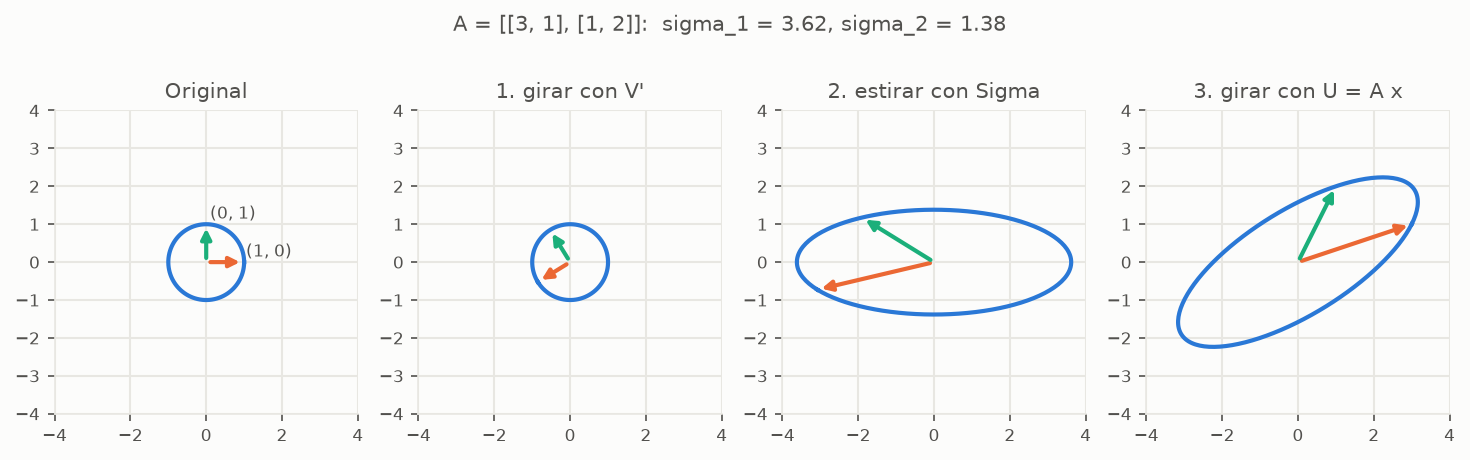
\includegraphics[width=\linewidth]{svd_geometria.png}
\caption{La SVD de $A = \left(\begin{smallmatrix} 3 & 1 \\ 1 & 2
\end{smallmatrix}\right)$ aplicada al círculo unitario, paso por paso.
Es el ejemplo gráfico de la exposición de clase.}
\label{fig:svd}
\end{figure}

\subsection*{Cómo se calcula a mano}

La idea clave es no atacar $A$ directamente, sino $A\T A$, que
\textbf{siempre} es cuadrada y simétrica, y a la que ya se le saben
sacar eigenvalores y eigenvectores. Ejemplo:
\[
    A = \begin{pmatrix} 1 & 0 \\ 0 & 1 \\ 1 & 1 \end{pmatrix},
    \qquad 3 \times 2 .
\]

\paragraph{Paso 1: $A\T A$.} Ya se calculó en la sección de
herramientas:
\[
    A\T A = \begin{pmatrix} 2 & 1 \\ 1 & 2 \end{pmatrix} .
\]

\paragraph{Paso 2: eigenvalores de $A\T A$.} También se calcularon:
$\lambda_1 = 3$ y $\lambda_2 = 1$, siempre de mayor a menor.

\paragraph{Paso 3: valores singulares.} Son las raíces de los
eigenvalores:
\[
    \sigma_1 = \raiz{3} = 1.732, \qquad \sigma_2 = \raiz{1} = 1,
    \qquad
    \Sigma = \begin{pmatrix} 1.732 & 0 \\ 0 & 1 \\ 0 & 0
             \end{pmatrix} .
\]
$\Sigma$ tiene el mismo tamaño que $A$.

\paragraph{Paso 4: $V$.} Los eigenvectores de $A\T A$, normalizados:
\[
    (1, 1) \to \frac{(1, 1)}{\raiz{2}} = (0.707,\ 0.707) = v_1,
    \qquad
    (1, -1) \to (0.707,\ -0.707) = v_2,
\]
\[
    V = \begin{pmatrix} 0.707 & 0.707 \\ 0.707 & -0.707 \end{pmatrix} .
\]

\paragraph{Paso 5: $U$ con $u = A v / \sigma$.}
\begin{align*}
    A v_1 &= \begin{pmatrix} 1 & 0 \\ 0 & 1 \\ 1 & 1 \end{pmatrix}
             \begin{pmatrix} 0.707 \\ 0.707 \end{pmatrix}
           = \begin{pmatrix} 0.707 \\ 0.707 \\ 1.414 \end{pmatrix},
    & u_1 &= \frac{A v_1}{1.732}
           = \begin{pmatrix} 0.408 \\ 0.408 \\ 0.816 \end{pmatrix}, \\
    A v_2 &= \begin{pmatrix} 0.707 \\ -0.707 \\ 0 \end{pmatrix},
    & u_2 &= \frac{A v_2}{1}
           = \begin{pmatrix} 0.707 \\ -0.707 \\ 0 \end{pmatrix} .
\end{align*}

\paragraph{Paso 6: completar $U$.} $U$ debe ser de $3 \times 3$ y
faltan columnas. La tercera es cualquier vector de largo 1
perpendicular a $u_1$ y $u_2$. Se encuentra resolviendo $A\T u = 0$:
\[
    \begin{pmatrix} 1 & 0 & 1 \\ 0 & 1 & 1 \end{pmatrix}
    \begin{pmatrix} x \\ y \\ z \end{pmatrix} = 0
    \;\Rightarrow\;
    x + z = 0,\ y + z = 0
    \;\Rightarrow\;
    u_3 = \frac{(1,\ 1,\ -1)}{\raiz{3}} .
\]
No afecta el resultado, porque en $\Sigma$ le toca la fila de ceros.

\paragraph{Paso 7: comprobar.} $U\Sigma$ son las dos primeras columnas
de $U$ multiplicadas por $\sigma_1$ y $\sigma_2$:
\[
    U \Sigma V\T =
    \begin{pmatrix} 0.707 & 0.707 \\ 0.707 & -0.707 \\ 1.414 & 0
    \end{pmatrix}
    \begin{pmatrix} 0.707 & 0.707 \\ 0.707 & -0.707 \end{pmatrix}
    =
    \begin{pmatrix} 1 & 0 \\ 0 & 1 \\ 1 & 1 \end{pmatrix} = A .
\]

\begin{resultado}
    El procedimiento a mano:
    \begin{enumerate}[itemsep=0.1em]
        \item calcular $A\T A$;
        \item sus eigenvalores $\lambda$, de mayor a menor;
        \item $\sigma = \raiz{\lambda}$, en la diagonal de $\Sigma$;
        \item sus eigenvectores normalizados, columnas de $V$;
        \item $u = A v / \sigma$, columnas de $U$;
        \item completar $U$ con vectores perpendiculares si hace falta.
    \end{enumerate}
\end{resultado}

\subsection*{Por qué funciona}

\paragraph{Por qué $A\T A$.} Si ya se supiera que $A = U \Sigma V\T$,
entonces
\[
    A\T A = (U \Sigma V\T)\T (U \Sigma V\T)
          = V \Sigma\T U\T U \Sigma V\T
          = V (\Sigma\T \Sigma) V\T ,
\]
porque $U\T U = I$. $\Sigma\T \Sigma$ es diagonal con los $\sigma^2$.
Esa expresión es una diagonalización de $A\T A$: las columnas de $V$
son sus eigenvectores y sus eigenvalores son los $\sigma^2$. De ahí
$\sigma = \raiz{\lambda}$.

\paragraph{Por qué la raíz siempre existe.} Si $v$ es eigenvector de
$A\T A$ y mide 1,
\[
    \lambda = v\T (A\T A) v = (A v)\T (A v) = \norm{A v}^2 \geq 0 .
\]
Un largo al cuadrado nunca es negativo.

\paragraph{Por qué $V$ y $U$ salen ortogonales.} $A\T A$ es simétrica,
así que sus eigenvectores son perpendiculares (teorema espectral). Para
$U$:
\[
    u_1 \cdot u_2
    = \frac{(A v_1) \cdot (A v_2)}{\sigma_1 \sigma_2}
    = \frac{v_1\T (A\T A v_2)}{\sigma_1 \sigma_2}
    = \frac{\sigma_2^2\, (v_1 \cdot v_2)}{\sigma_1 \sigma_2} = 0 ,
\]
y cada $u$ mide 1 porque $\norm{A v} = \sigma$.

\paragraph{Por qué el producto da $A$.} De $u = A v / \sigma$ sale
$A v_i = \sigma_i u_i$. Juntando todas las columnas, $A V = U \Sigma$;
y como $V^{-1} = V\T$, queda $A = U \Sigma V\T$.

\subsection*{La SVD como suma de piezas de rango 1}

Multiplicando por bloques, la SVD también se escribe como una suma:
\[
    A = \sigma_1\, u_1 v_1\T + \sigma_2\, u_2 v_2\T + \cdots
\]
Cada $u_i v_i\T$ es una columna por una fila: una matriz de rango 1.
Como los $\sigma$ vienen ordenados, la primera pieza es la que más
pesa.

\begin{teorema}[Eckart-Young]
    Quedarse con las primeras $k$ piezas da la \textbf{mejor
    aproximación de rango $k$} de $A$: ninguna otra matriz de rango $k$
    queda más cerca. Lo que se pierde son los $\sigma$ que se tiraron:
    \[
        \norm{A - A_k}^2 = \sigma_{k+1}^2 + \sigma_{k+2}^2 + \cdots
    \]
\end{teorema}

\begin{ejemplo}
    En el ejemplo, con $k = 1$:
    \[
        A_1 = \sigma_1 u_1 v_1\T
            = 1.732
              \begin{pmatrix} 0.408 \\ 0.408 \\ 0.816 \end{pmatrix}
              \begin{pmatrix} 0.707 & 0.707 \end{pmatrix}
            = \begin{pmatrix} 0.5 & 0.5 \\ 0.5 & 0.5 \\ 1 & 1
              \end{pmatrix} .
    \]
    El error al cuadrado es $\sigma_2^2 = 1$, de una energía total
    $\sigma_1^2 + \sigma_2^2 = 4$: con una sola pieza se conserva el
    75\,\%.
\end{ejemplo}

\subsection*{Qué pieza usa K-SVD}

K-SVD usa solo la \textbf{primera pieza}. Al actualizar un átomo arma
una matriz $R$ con lo que ese átomo tiene que explicar en cada ventana
y se pregunta qué átomo, por qué pesos, explica mejor a $R$. Un átomo
por sus pesos es columna por fila, rango 1, y la mejor respuesta de
rango 1 es la primera pieza de la SVD:
\[
    \text{átomo nuevo} = u_1,
    \qquad
    \text{pesos nuevos} = \sigma_1\, v_1 .
\]

\begin{ojo}
    \textbf{El signo es arbitrario.} Si se cambia el signo de $u_i$ y
    de $v_i$ a la vez, el producto no cambia. Por eso numpy a veces
    devuelve los vectores con el signo contrario al de las cuentas a
    mano, y es la misma solución. Además, \texttt{np.linalg.svd} no
    forma $A\T A$, porque esa multiplicación pierde precisión; usa otro
    método (bidiagonalización de Golub-Kahan). La matemática es la
    misma, solo cambia cómo se hacen las cuentas.
\end{ojo}

\newpage

% =====================================================================
%  6. OMP
% =====================================================================

\section{OMP: cómo cada ventana escoge sus átomos}

\begin{quick_sum}
    Con el diccionario fijo, OMP encuentra para cada ventana unos pocos
    átomos y sus pesos. Escoge un átomo a la vez, el que más se parece
    a lo que falta explicar, y en cada vuelta reajusta los pesos de
    todos los escogidos. Es el paso 1 de K-SVD, y lo único que produce
    es $\alpha$.
\end{quick_sum}

\subsection*{El problema}

Con el diccionario fijo, para cada ventana $x$ se busca $\alpha$ tal
que $x = D\alpha$. Son 128 ecuaciones y 256 incógnitas: hay
\textbf{infinitas} soluciones, y se quiere la que tenga \textbf{más
ceros}.

Encontrar la mejor exacta es carísimo: habría que probar todas las
combinaciones de átomos. Solo para escoger 8 átomos de 256 hay
\[
    \binom{256}{8} \approx 4.1 \times 10^{14}
\]
combinaciones. OMP la aproxima de forma \textbf{voraz}: escoge un átomo
a la vez, el que más ayuda en ese momento, sin volver atrás.

\subsection*{El algoritmo}

\begin{algorithm}[H]
\caption{Orthogonal Matching Pursuit sobre una ventana}
\begin{algorithmic}[1]
    \Require diccionario $D$, ventana $x$, error objetivo $\varepsilon$,
             tope $k$
    \Ensure pesos $\alpha$ con pocas entradas distintas de cero
    \State $r \gets x$ \Comment{al inicio falta explicar todo}
    \State $S \gets \emptyset$ \Comment{átomos escogidos}
    \While{$\norm{r} / \norm{x} > \varepsilon$ \textbf{y} $|S| < k$}
        \State calcular $|d_i \cdot r|$ para cada átomo $i$
        \State $S \gets S \cup \{\text{el átomo con el valor
               mayor}\}$
        \State $w \gets$ pesos de mínimos cuadrados con los átomos
               de $S$
        \State $r \gets x - D_S\, w$
    \EndWhile
    \State \Return $\alpha$, con $w$ en los átomos de $S$ y cero en
           los demás
\end{algorithmic}
\end{algorithm}

En el proyecto, $\varepsilon = 0.1$ (\texttt{ERROR\_OMP}) y $k = 16$
(\texttt{MAX\_ATOMOS\_OMP}). Por qué cada paso:

\begin{itemize}[itemsep=0.3em]
    \item \textbf{Comparar con el residual.} El producto punto mide
          parecido; como todos los átomos miden 1, el de valor absoluto
          mayor es el que mejor explica lo que falta. Se usa valor
          absoluto porque un átomo al revés, con peso negativo, explica
          igual.
    \item \textbf{Reajustar todos los pesos.} No solo se calcula el
          peso del átomo nuevo: se recalculan los de todos los
          escogidos. Eso es lo \textbf{ortogonal} del nombre, y hace
          que ningún átomo se repita.
    \item \textbf{Siempre contra lo que falta.} La comparación es
          contra el residual $r$, no contra la ventana original.
\end{itemize}

\subsection*{Los mínimos cuadrados del paso de pesos}

Con los átomos escogidos se buscan los pesos que dejan la suma lo más
cerca posible de $x$. ¿Cómo se reconocen esos pesos? Por una propiedad:
\textbf{lo que sobra no debe parecerse a ningún átomo escogido}. Si se
pareciera a alguno, se podría mover su peso para explicar ese pedazo y
el residual bajaría. Entonces el residual debe ser perpendicular a cada
átomo escogido. Con dos átomos $P$ y $Q$:
\[
    P \cdot (x - w_P P - w_Q Q) = 0, \qquad
    Q \cdot (x - w_P P - w_Q Q) = 0 .
\]
Esas dos condiciones son todo. Falta despejarlas. Se reparte el
producto punto, que se distribuye igual que una multiplicación normal:
\[
    P \cdot x - w_P\,(P \cdot P) - w_Q\,(P \cdot Q) = 0 ,
\]
y pasando a la derecha lo que no tiene incógnita:
\[
    w_P\,(P \cdot P) + w_Q\,(P \cdot Q) = P \cdot x .
\]
Lo mismo con la segunda condición. Son dos ecuaciones con dos
incógnitas, y puestas en forma de matriz se llaman las
\textbf{ecuaciones normales}:
\[
    \begin{pmatrix} P \cdot P & P \cdot Q \\ Q \cdot P & Q \cdot Q
    \end{pmatrix}
    \begin{pmatrix} w_P \\ w_Q \end{pmatrix}
    =
    \begin{pmatrix} P \cdot x \\ Q \cdot x \end{pmatrix} .
\]
Cada renglón dice lo mismo: \emph{el átomo de este renglón, contra lo
reconstruido, debe dar lo mismo que ese átomo contra $x$}.

\textbf{El caso de un solo átomo.} Con un átomo $P$ el sistema se
encoge a $1 \times 1$ y queda una sola ecuación:
\[
    (P \cdot P)\, w_P = P \cdot x .
\]
Y aquí entra un detalle del montaje: \textbf{los átomos están
normalizados a norma 1}, así que $P \cdot P = \norm{P}^2 = 1$. El
sistema se vuelve $1 \cdot w_P = P \cdot x$, o sea
\[
    w_P = P \cdot x .
\]
El peso del primer átomo \emph{es} su producto punto con la ventana.
Por eso en el ejemplo el 1.4 aparece dos veces: primero como el
producto punto que hizo ganar a $B$, y después como su peso. No es
coincidencia, es la misma cuenta.

\begin{idea}
    Si los átomos son perpendiculares ($P \cdot Q = 0$) y miden 1, la
    matriz es la identidad y cada peso es simplemente su producto punto
    con $x$. Si \textbf{no} son perpendiculares, hay que resolver el
    sistema y los pesos se reparten. En el código esto es una línea,
    \texttt{np.linalg.lstsq}.
\end{idea}

\subsection*{Ejemplo completo: la ventana 1}

La ventana es $x = v_1 = (1,\ 1,\ 0.5)$, con
$\norm{x} = \raiz{1 + 1 + 0.25} = 1.5$, y el objetivo es error menor a
0.1. Al inicio el residual es la ventana completa:
$r = (1,\ 1,\ 0.5)$. La figura~\ref{fig:omp} resume las tres vueltas.

\begin{figure}[H]
\centering
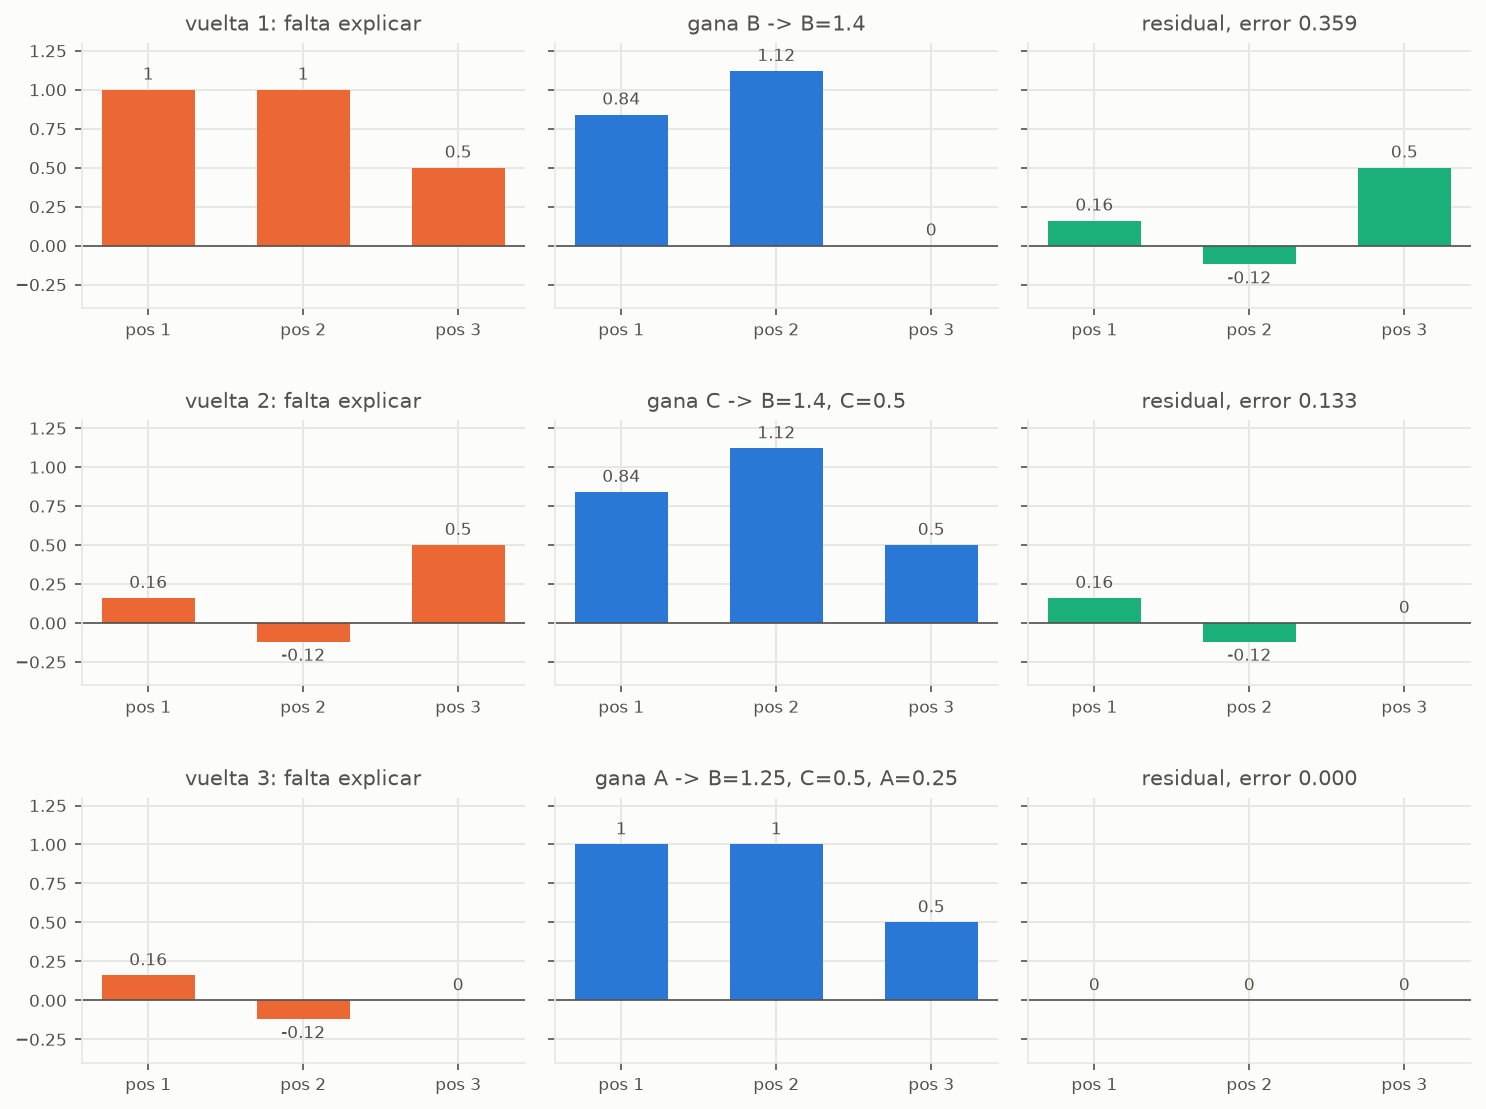
\includegraphics[width=0.92\linewidth]{omp_vueltas.png}
\caption{OMP sobre la ventana 1. En cada fila: lo que falta explicar
antes de la vuelta (naranja), la reconstrucción después (azul) y el
residual que queda (verde).}
\label{fig:omp}
\end{figure}

\subsubsection*{Vuelta 1}

\textbf{Comparar cada átomo con el residual:}
\begin{align*}
    \cA{A} \cdot r &= (1)(1) + (0)(1) + (0)(0.5) = 1 \\
    \cB{B} \cdot r &= (0.6)(1) + (0.8)(1) + (0)(0.5) = 1.4 \\
    \cC{C} \cdot r &= (0)(1) + (0)(1) + (1)(0.5) = 0.5 \\
    \cE{E} \cdot r &= (0)(1) + (1)(1) + (0)(0.5) = 1
\end{align*}
El mayor es 1.4: gana \cB{$B$}. Escogidos: $\{B\}$.

\textbf{Peso.} Hay un solo átomo escogido, así que las ecuaciones
normales se reducen a una sola:
\[
    (B \cdot B)\, w_B = B \cdot x .
\]
El lado izquierdo es $B \cdot B = (0.6)^2 + (0.8)^2 + 0^2 = 1$, porque
los átomos se construyeron con norma 1. El derecho ya se calculó
arriba: $B \cdot x = 1.4$. Entonces $1 \cdot w_B = 1.4$ y
$w_B = 1.4$.

En otras palabras, el peso salió gratis: el producto punto que se usó
para \emph{elegir} el átomo sirve también como su \emph{peso}. Eso
solo pasa con el primer átomo, cuando no hay otros con los cuales
repartirse la explicación.

\textbf{Reconstrucción y residual:}
\[
    1.4\, B = (0.84,\ 1.12,\ 0),
    \qquad
    r = x - 1.4\, B = (1 - 0.84,\ 1 - 1.12,\ 0.5 - 0)
      = (0.16,\ -0.12,\ 0.5) .
\]

\textbf{Error:}
\[
    \norm{r} = \raiz{0.16^2 + 0.12^2 + 0.5^2}
             = \raiz{0.0256 + 0.0144 + 0.25} = \raiz{0.29} = 0.539,
    \qquad
    \frac{0.539}{1.5} = 0.359 > 0.1 .
\]
Sigue.

\subsubsection*{Vuelta 2}

\textbf{Comparar con el residual nuevo,} $r = (0.16,\ -0.12,\ 0.5)$:
\begin{align*}
    \cA{A} \cdot r &= 0.16 \\
    \cB{B} \cdot r &= (0.6)(0.16) + (0.8)(-0.12) = 0.096 - 0.096 = 0 \\
    \cC{C} \cdot r &= 0.5 \\
    \cE{E} \cdot r &= -0.12
\end{align*}
$B$ da \textbf{cero}: lo que sobra ya no tiene nada de $B$, y así se
garantiza que no se repite. Gana \cC{$C$}, que tiene sentido: lo que
más faltaba era el 0.5 de la tercera posición. Escogidos: $\{B, C\}$.

\textbf{Pesos de $B$ y $C$ juntos.} Aquí hay un punto que se presta a
confusión. Los productos punto del lado derecho van contra la $x$
\textbf{original}, no contra el residual, aunque el residual sea lo
que se acaba de usar para escoger a $C$.

La razón es que son dos preguntas distintas. El residual contesta
\emph{cuál átomo entra}: es lo que falta por explicar, y se busca el
átomo que más se le parezca. Pero una vez elegido el conjunto, la
pregunta cambia a \emph{con qué pesos}, y esa se responde minimizando
$\norm{x - w_B B - w_C C}$, que habla de $x$ y no del residual de la
vuelta anterior. Las ecuaciones normales salen de ahí, así que su lado
derecho tiene que ser $B \cdot x$ y $C \cdot x$.

Esto es justamente lo \emph{ortogonal} de Orthogonal Matching Pursuit:
en cada vuelta se recalculan \textbf{todos} los pesos desde cero,
incluidos los de los átomos viejos, en lugar de dejarlos fijos y solo
agregar el nuevo. Los números:
\[
    B \cdot B = 1,\quad B \cdot C = 0,\quad C \cdot C = 1,\quad
    B \cdot x = 1.4,\quad C \cdot x = 0.5,
\]
\[
    \begin{pmatrix} 1 & 0 \\ 0 & 1 \end{pmatrix}
    \begin{pmatrix} w_B \\ w_C \end{pmatrix}
    = \begin{pmatrix} 1.4 \\ 0.5 \end{pmatrix}
    \;\Rightarrow\; w_B = 1.4,\ w_C = 0.5 .
\]
Como $B$ y $C$ son perpendiculares, cada ecuación tiene una sola
incógnita y el peso de $B$ no cambia.

\textbf{Reconstrucción, residual y error:}
\[
    1.4\, B + 0.5\, C = (0.84,\ 1.12,\ 0.5),
    \qquad
    r = (0.16,\ -0.12,\ 0),
    \qquad
    \frac{\raiz{0.04}}{1.5} = \frac{0.2}{1.5} = 0.133 > 0.1 .
\]
Sigue.

\subsubsection*{Vuelta 3}

\textbf{Comparar,} $r = (0.16,\ -0.12,\ 0)$:
\[
    \cA{A} \cdot r = 0.16, \qquad
    \cB{B} \cdot r = 0, \qquad
    \cC{C} \cdot r = 0, \qquad
    \cE{E} \cdot r = -0.12 .
\]
Gana \cA{$A$}. Escogidos: $\{B, C, A\}$.

\textbf{Pesos de los tres.} Ahora hay tres átomos escogidos, así que
el sistema crece a $3 \times 3$. En el orden $B$, $C$, $A$ queda:
\[
    \begin{pmatrix}
        B \cdot B & B \cdot C & B \cdot A \\
        C \cdot B & C \cdot C & C \cdot A \\
        A \cdot B & A \cdot C & A \cdot A
    \end{pmatrix}
    \begin{pmatrix} w_B \\ w_C \\ w_A \end{pmatrix}
    =
    \begin{pmatrix} B \cdot x \\ C \cdot x \\ A \cdot x \end{pmatrix} .
\]
Son nueve casillas en la matriz y tres en el lado derecho, pero
\textbf{cinco ya se calcularon en la vuelta 2} y se reusan:
$B \cdot B = 1$, $B \cdot C = 0$, $C \cdot C = 1$, $B \cdot x = 1.4$,
$C \cdot x = 0.5$. Y la matriz es simétrica, porque el producto punto
no distingue el orden: $A \cdot B$ es lo mismo que $B \cdot A$. Así
que solo faltan cuatro números, los que involucran al átomo nuevo:
\[
    B \cdot A = (0.6)(1) + (0.8)(0) + (0)(0) = 0.6,
    \qquad C \cdot A = (0)(1) + (0)(0) + (1)(0) = 0,
\]
\[
    A \cdot A = (1)(1) + (0)(0) + (0)(0) = 1,
    \qquad A \cdot x = (1)(1) + (0)(1) + (0)(0.5) = 1 .
\]

\textbf{Aquí está lo importante: $B \cdot A = 0.6$, distinto de
cero.} $A$ y $B$ \textbf{no} son perpendiculares, y por eso esta
vuelta es la primera en que el sistema de verdad hay que resolverlo.
Sustituyendo los números:
\[
    \begin{pmatrix}
        1   & 0 & 0.6 \\
        0   & 1 & 0   \\
        0.6 & 0 & 1
    \end{pmatrix}
    \begin{pmatrix} w_B \\ w_C \\ w_A \end{pmatrix}
    =
    \begin{pmatrix} 1.4 \\ 0.5 \\ 1 \end{pmatrix} .
\]

\textbf{Pasarlo a ecuaciones.} Una matriz por un vector es, renglón
por renglón, un producto punto. El primer renglón $(1,\ 0,\ 0.6)$
contra $(w_B,\ w_C,\ w_A)$ da
$1 \cdot w_B + 0 \cdot w_C + 0.6 \cdot w_A$, y eso debe igualar al
primer número de la derecha. Los tres renglones:
\[
    \begin{aligned}
        w_B + 0\,w_C + 0.6\, w_A &= 1.4 && (1) \\
        0\,w_B + w_C + 0\,w_A    &= 0.5 && (2) \\
        0.6\, w_B + 0\,w_C + w_A &= 1   && (3)
    \end{aligned}
    \qquad\Longleftrightarrow\qquad
    \begin{aligned}
        w_B + 0.6\, w_A &= 1.4 && (1) \\
        w_C &= 0.5 && (2) \\
        0.6\, w_B + w_A &= 1 && (3)
    \end{aligned}
\]
Los ceros se van, y lo que queda deja ver la estructura: la ecuación
(2) está sola, y las otras dos están enredadas entre sí.

\textbf{Resolver.} La (2) ya viene despejada: $w_C = 0.5$. Tiene
sentido, $C$ es perpendicular a los otros dos, así que nadie compite
con él y se queda con su producto punto completo.

Quedan (1) y (3), dos ecuaciones con dos incógnitas. Se despeja $w_A$
de la (3), que es la más directa:
\[
    0.6\, w_B + w_A = 1
    \qquad\Longrightarrow\qquad
    w_A = 1 - 0.6\, w_B .
\]
Y esa expresión se mete en la (1), donde aparecía $w_A$, para que
quede una sola incógnita:
\begin{align*}
    w_B + 0.6\, w_A            &= 1.4
        && \text{ecuación (1)} \\
    w_B + 0.6\,(1 - 0.6\, w_B) &= 1.4
        && \text{se sustituye } w_A \\
    w_B + 0.6 - 0.36\, w_B     &= 1.4
        && \text{se reparte el } 0.6 \\
    0.64\, w_B                 &= 0.8
        && \text{se juntan los } w_B \text{ y pasa el } 0.6 \\
    w_B                        &= \frac{0.8}{0.64} = 1.25 .
\end{align*}
Con $w_B$ ya conocido, se regresa a la expresión de $w_A$:
\[
    w_A = 1 - 0.6 \cdot 1.25 = 1 - 0.75 = 0.25 .
\]

\begin{ojo}
    \textbf{El peso de $B$ cambió de 1.4 a 1.25.} En la vuelta 1, $B$
    explicaba sola la primera posición. Ahora $A$ también aporta ahí,
    así que $B$ ya no carga con todo. Si los pesos se sacaran con un
    producto punto cada uno, saldría $w_B = 1.4$ y $w_A = 1$, y la
    reconstrucción quedaría mal.
\end{ojo}

\textbf{Reconstrucción, residual y error:}
\[
    1.25\, B + 0.5\, C + 0.25\, A
    = (0.75,\ 1,\ 0) + (0,\ 0,\ 0.5) + (0.25,\ 0,\ 0)
    = (1,\ 1,\ 0.5) = x .
\]
El residual es $r = 0$ y el error es 0: se detiene.

\begin{resultado}
    \[
        \alpha^{(1)} = (\,\cA{0.25},\ \cB{1.25},\ \cC{0.5},\ \cE{0}\,)
    \]
    \begin{center}
    \begin{tabular}{cccc}
        \toprule
        \textbf{Vuelta} & \textbf{Gana} & \textbf{Pesos}
                        & \textbf{Error} \\
        \midrule
        1 & $B$ & $B = 1.4$                         & 0.359 \\
        2 & $C$ & $B = 1.4,\ C = 0.5$               & 0.133 \\
        3 & $A$ & $B = 1.25,\ C = 0.5,\ A = 0.25$   & 0 \\
        \bottomrule
    \end{tabular}
    \end{center}
\end{resultado}

\subsection*{La ventana 2}

La ventana es $x = v_2 = (0.9,\ 1,\ 0)$, con
$\norm{x} = \raiz{0.81 + 1} = 1.345$.

\textbf{Vuelta 1.} Comparar con $r = x$:
\[
    \cA{A} \cdot r = 0.9, \qquad
    \cB{B} \cdot r = 0.54 + 0.8 = 1.34, \qquad
    \cC{C} \cdot r = 0, \qquad
    \cE{E} \cdot r = 1 .
\]
Gana \cB{$B$} con peso $w_B = 1.34$. Reconstrucción y residual:
\[
    1.34\, B = (0.804,\ 1.072,\ 0),
    \qquad
    r = (0.096,\ -0.072,\ 0),
    \qquad
    \frac{\raiz{0.0092 + 0.0052}}{1.345} = \frac{0.12}{1.345}
    = 0.089 < 0.1 .
\]
Se detiene con un solo átomo: no queda exacta, pero ya cumple el
objetivo. $\alpha^{(2)} = (0,\ 1.34,\ 0,\ 0)$.

\subsection*{Lo que hay que recordar}

\begin{enumerate}[itemsep=0.3em]
    \item Se compara contra \textbf{lo que falta}, no contra la ventana
          original. Por eso en la vuelta 2 gana $C$, aunque al inicio
          era el que menos se parecía.
    \item Un átomo ya escogido da \textbf{cero} en las vueltas
          siguientes. Nunca se repite.
    \item Los pesos viejos \textbf{se reajustan}: $B$ pasó de 1.4 a
          1.25.
    \item Para en cuanto basta: error menor a 0.1 o 16 átomos.
    \item Lo único que produce OMP es $\alpha$. El diccionario no
          cambia.
\end{enumerate}

\newpage

% =====================================================================
%  7. Actualización de átomos
% =====================================================================

\section{Actualización de átomos: el paso de la SVD}

\begin{quick_sum}
    Con los pesos de OMP fijos, se recorre cada átomo en orden. Se
    juntan las ventanas que lo usan, se les quita lo que explican los
    demás átomos, y a esa matriz se le saca la SVD: el átomo nuevo es
    $u_1$ y sus pesos nuevos son $\sigma_1 v_1$. En el ejemplo, el
    error total baja de 0.12 a 0.056.
\end{quick_sum}

\subsection*{Punto de partida}

Del ejemplo de juguete y de OMP se tienen:
\[
    D = \begin{pmatrix}
        \cA{1} & \cB{0.6} & \cC{0} & \cE{0} \\
        \cA{0} & \cB{0.8} & \cC{0} & \cE{1} \\
        \cA{0} & \cB{0}   & \cC{1} & \cE{0}
    \end{pmatrix},
    \qquad
    X = \begin{pmatrix} 1 & 0.9 \\ 1 & 1 \\ 0.5 & 0 \end{pmatrix},
    \qquad
    \alpha = \begin{pmatrix}
        0.25 & 0    \\
        1.25 & 1.34 \\
        0.5  & 0    \\
        0    & 0
    \end{pmatrix} .
\]
Con esto la ventana 1 sale exacta y a la ventana 2 le falta
$(0.096,\ -0.072,\ 0)$: el error total es 0.12.

\subsection*{Qué quiere hacer este paso}

OMP decidió \textbf{qué átomos usa cada ventana}. Ahora se cambia la
pregunta: con esas decisiones fijas, ¿se pueden mejorar los átomos? Se
revisa un átomo a la vez, \textbf{en orden}: $A$, $B$, $C$, $E$. Para
cada uno, la pregunta es: si dejo fijos los demás átomos, ¿qué forma
debería tener este átomo, y con qué pesos, para explicar lo mejor
posible las ventanas que lo usan?

\begin{ojo}
    \textbf{Solo se miran las ventanas que ya usan el átomo.} Si se
    miraran todas, el átomo entraría en ventanas que no lo tenían y se
    perderían los ceros que OMP acababa de construir.
\end{ojo}

\subsection*{De dónde sale el residual}

Tomemos el átomo $j$ y las ventanas $w$ que lo usan. Cada una de esas
ventanas se reconstruye sumando varios átomos, y uno de los sumandos
es el que estamos por cambiar:
\[
    \text{ventana} \;\approx\;
    \underbrace{\text{lo que aportan los otros átomos}}
               _{\text{se queda fijo}}
    \;+\;
    \underbrace{\alpha_{j,\ell}\, d_j}_{\text{esto se va a cambiar}} .
\]
Si la parte fija se queda como está, lo único que el átomo $j$ puede
mejorar es \textbf{lo que sobra después de restarla}. Eso es el
residual:
\[
    R = X_w - D\,\alpha_w ,
    \qquad \text{con la fila } j \text{ de } \alpha_w \text{ en cero.}
\]
Poner esa fila en cero es la forma de decir \emph{apaga el átomo $j$ y
déjame ver qué queda}. Si no se apagara, se estaría restando la
contribución vieja del átomo, y el residual sería lo que falta
\emph{además} de lo que $j$ ya hacía, que no es lo que se quiere
mejorar.

\subsection*{Por qué la respuesta es una SVD}

Ya con $R$, la pregunta es: ¿qué átomo $d_j$ y qué pesos $\alpha_j$
dejan $d_j \alpha_j\T$ lo más parecido posible a $R$?

Y ahí está el truco. $d_j$ es una columna y $\alpha_j$ una fila, así
que su producto es una \textbf{matriz de rango 1}, siempre, sin
importar qué valores tengan. Entonces la pregunta se traduce sola:
\begin{center}
    \emph{¿cuál es la mejor aproximación de rango 1 de $R$?}
\end{center}
Esa pregunta ya tiene respuesta, y es el teorema de Eckart-Young de la
sección anterior: la mejor aproximación de rango 1 es
$\sigma_1 u_1 v_1\T$. Comparando término a término:
\[
    d_j \alpha_j\T = \sigma_1\, u_1 v_1\T
    \qquad\Longrightarrow\qquad
    d_j = u_1 , \quad \alpha_j = \sigma_1\, v_1 .
\]
El átomo se queda con $u_1$ y el factor $\sigma_1$ se va a los pesos.
El reparto es así y no al revés porque $u_1$ ya tiene norma 1, que es
la condición que deben cumplir los átomos; si se le colgara el
$\sigma_1$ al átomo, habría que renormalizarlo y el paso dejaría de
ser el óptimo.

\begin{idea}
    No se está \emph{eligiendo} usar una SVD por conveniencia. La
    forma del problema, columna por fila, obliga a que la solución sea
    de rango 1, y para ese problema la SVD \textbf{es} la respuesta
    exacta. De ahí el nombre del algoritmo: una SVD por átomo, en cada
    iteración.
\end{idea}

\begin{algorithm}[H]
\caption{Actualización del átomo $j$}
\begin{algorithmic}[1]
    \Require diccionario $D$, ventanas $X$, pesos $\alpha$, átomo $j$
    \State $w \gets$ ventanas con $\alpha_{j,\ell} \neq 0$
           \Comment{la fila $j$ de $\alpha$}
    \If{$w$ está vacío}
        \State $d_j \gets$ la ventana peor reconstruida, normalizada
        \State \Return
    \EndIf
    \State $R \gets X_w - D\,\alpha_w$, con la fila $j$ de $\alpha_w$
           en cero \Comment{lo que $d_j$ debe explicar}
    \State $U, \Sigma, V\T \gets \operatorname{SVD}(R)$
    \State $d_j \gets u_1$
    \State $\alpha_{j, w} \gets \sigma_1\, v_1\T$
\end{algorithmic}
\end{algorithm}

\subsection*{Átomo $A$}

\textbf{Qué ventanas lo usan.} La fila $A$ de $\alpha$ es
$(0.25,\ 0)$: solo la ventana 1.

\textbf{Residual.} A la ventana 1 se le quita lo que aportan los otros
átomos que usa, $B$ y $C$:
\[
    R = v_1 - (1.25\, B + 0.5\, C)
      = (1,\ 1,\ 0.5) - (0.75,\ 1,\ 0) - (0,\ 0,\ 0.5)
      = (0.25,\ 0,\ 0) .
\]
Como solo una ventana usa $A$, $R$ es una matriz de \textbf{una
columna}.

\textbf{SVD de una sola columna.} Es el caso más simple:
$R\T R = 0.25^2 = 0.0625$ es un solo número, su eigenvalor es él mismo,
$\sigma = \raiz{0.0625} = 0.25 = \norm{R}$, $v = (1)$, y
\[
    u = \frac{R\, v}{\sigma} = \frac{(0.25,\ 0,\ 0)}{0.25}
      = (1,\ 0,\ 0) .
\]
Con una sola columna la SVD siempre da $u = R / \norm{R}$ y
$\sigma = \norm{R}$.

\textbf{Actualizar.} $A$ nuevo $= (1,\ 0,\ 0)$ y su peso es 0.25:
\textbf{no cambia}, porque lo que le tocaba explicar ya apuntaba
exactamente en su dirección.

\subsection*{Átomo $B$}

Es el caso interesante, porque lo usan \textbf{dos} ventanas.

\textbf{Qué ventanas lo usan.} La fila $B$ de $\alpha$ es
$(1.25,\ 1.34)$: las dos.

\textbf{Residual de cada ventana.} A la ventana 1 se le quitan $A$ y
$C$; la ventana 2 solo usa $B$, así que no se le quita nada:
\begin{align*}
    R_1 &= (1,\ 1,\ 0.5) - (0.25,\ 0,\ 0) - (0,\ 0,\ 0.5)
         = (0.75,\ 1,\ 0), \\
    R_2 &= (0.9,\ 1,\ 0) .
\end{align*}
Como columnas:
\[
    R = \begin{pmatrix} 0.75 & 0.9 \\ 1 & 1 \\ 0 & 0 \end{pmatrix} .
\]

\textbf{Qué se busca.} Un átomo $b$ de largo 1 y dos pesos $(p_1, p_2)$
tales que $p_1 b \approx R_1$ y $p_2 b \approx R_2$; en forma de
matriz, $b\,(p_1\ p_2) \approx R$. Es columna por fila: rango 1. El $B$
viejo, $(0.6,\ 0.8,\ 0)$, no le queda perfecto a ninguna: $R_1$ y $R_2$
apuntan un poco más a la derecha. Se busca \textbf{una sola dirección}
que les quede lo mejor posible \textbf{a las dos a la vez}: la primera
pieza de la SVD de $R$.

\paragraph{Paso 1: $R\T R$.} Sus entradas son productos punto entre
las columnas de $R$:
\begin{align*}
    R_1 \cdot R_1 &= 0.75^2 + 1^2 = 0.5625 + 1 = 1.5625 \\
    R_1 \cdot R_2 &= 0.75 \cdot 0.9 + 1 \cdot 1 = 0.675 + 1 = 1.675 \\
    R_2 \cdot R_2 &= 0.9^2 + 1^2 = 0.81 + 1 = 1.81
\end{align*}
\[
    R\T R = \begin{pmatrix} 1.5625 & 1.675 \\ 1.675 & 1.81
            \end{pmatrix} .
\]

\paragraph{Paso 2: eigenvalores.} Para una de $2 \times 2$,
$\lambda^2 - (\text{traza})\,\lambda + \det = 0$:
\begin{align*}
    \text{traza} &= 1.5625 + 1.81 = 3.3725 \\
    \det &= 1.5625 \cdot 1.81 - 1.675^2 = 2.8281 - 2.8056 = 0.0225 \\
    \lambda &= \frac{3.3725 \pm \raiz{3.3725^2 - 4 \cdot 0.0225}}{2}
             = \frac{3.3725 \pm \raiz{11.2838}}{2}
             = \frac{3.3725 \pm 3.3591}{2} \\
    \lambda_1 &= 3.3658, \qquad \lambda_2 = 0.0067
\end{align*}

\paragraph{Paso 3: valores singulares.}
\[
    \sigma_1 = \raiz{3.3658} = 1.8346,
    \qquad
    \sigma_2 = \raiz{0.0067} = 0.0818 .
\]
$\sigma_1$ es unas 22 veces mayor que $\sigma_2$: $R_1$ y $R_2$
apuntan casi a la misma dirección. $\sigma_1$ explica
$3.3658 / 3.3725$, es decir el 99.8\,\% de la energía.

\paragraph{Paso 4: $v_1$.} Se resuelve
$(R\T R - \lambda_1 I)\, v = 0$:
\[
    \begin{pmatrix} -1.8033 & 1.675 \\ 1.675 & -1.5558 \end{pmatrix}
    \begin{pmatrix} a \\ b \end{pmatrix} = 0
    \;\Rightarrow\;
    b = \frac{1.8033}{1.675}\, a = 1.0766\, a .
\]
Con $a = 1$, $v = (1,\ 1.0766)$, de largo
$\raiz{1 + 1.1591} = 1.4694$. Normalizado:
$v_1 = (0.6806,\ 0.7327)$.

\paragraph{Paso 5: $u_1 = R v_1 / \sigma_1$.}
\[
    R v_1 =
    \begin{pmatrix}
        0.75 \cdot 0.6806 + 0.9 \cdot 0.7327 \\
        1 \cdot 0.6806 + 1 \cdot 0.7327 \\
        0
    \end{pmatrix}
    = \begin{pmatrix} 1.1698 \\ 1.4133 \\ 0 \end{pmatrix},
    \qquad
    u_1 = \frac{R v_1}{1.8346}
        = \begin{pmatrix} 0.6377 \\ 0.7703 \\ 0 \end{pmatrix} .
\]
Revisión: $\norm{u_1} = \raiz{0.4067 + 0.5934} = 1$.

\paragraph{Paso 6: qué se queda y qué se tira.} La primera pieza de la
SVD es
\[
    \sigma_1 u_1 v_1\T
    = 1.8346
      \begin{pmatrix} 0.6377 \\ 0.7703 \\ 0 \end{pmatrix}
      \begin{pmatrix} 0.6806 & 0.7327 \end{pmatrix}
    = \begin{pmatrix} 0.797 & 0.858 \\ 0.962 & 1.035 \\ 0 & 0
      \end{pmatrix}
    \quad\text{contra}\quad
    R = \begin{pmatrix} 0.75 & 0.9 \\ 1 & 1 \\ 0 & 0 \end{pmatrix} .
\]
Muy parecidas. La diferencia es lo que una sola dirección no puede
explicar, y mide exactamente $\sigma_2$:
\[
    R - \sigma_1 u_1 v_1\T =
    \begin{pmatrix} -0.047 & 0.042 \\ 0.038 & -0.035 \\ 0 & 0
    \end{pmatrix},
    \qquad
    \raiz{0.047^2 + 0.042^2 + 0.038^2 + 0.035^2} = 0.0818 = \sigma_2 .
\]

\paragraph{Paso 7: actualizar.}
\[
    B_{\text{nuevo}} = u_1 = (0.6377,\ 0.7703,\ 0),
    \qquad
    \text{pesos} = \sigma_1 v_1 = 1.8346\,(0.6806,\ 0.7327)
                 = (1.2486,\ 1.3442) .
\]

\begin{center}
\begin{tabular}{lcc}
    \toprule
                     & \textbf{Antes} & \textbf{Después} \\
    \midrule
    $B$              & $(0.6,\ 0.8,\ 0)$ & $(0.6377,\ 0.7703,\ 0)$ \\
    peso en $v_1$    & 1.25              & 1.2486 \\
    peso en $v_2$    & 1.34              & 1.3442 \\
    \bottomrule
\end{tabular}
\end{center}

\begin{figure}[H]
\centering
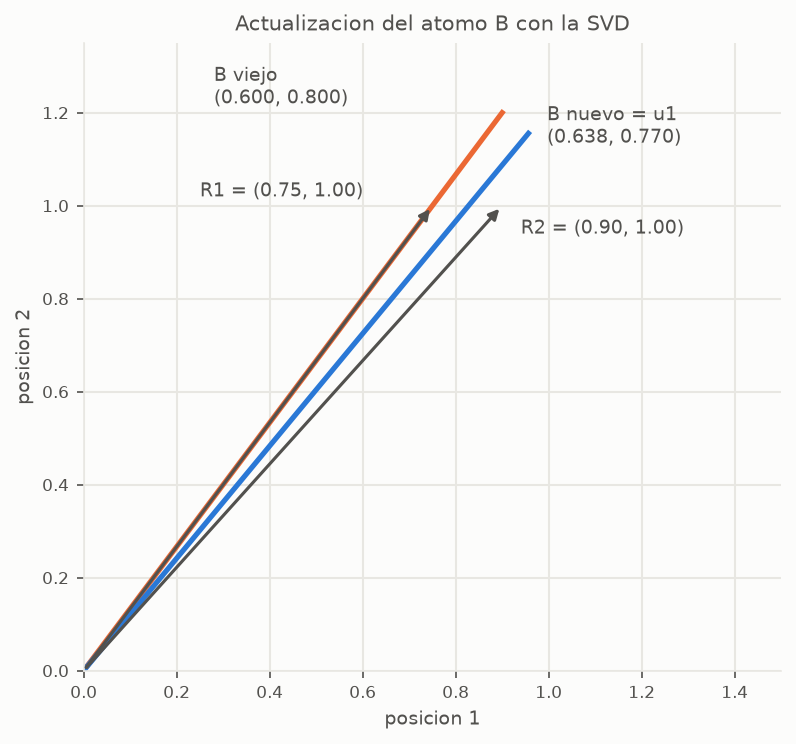
\includegraphics[width=0.62\linewidth]{actualizar_b.png}
\caption{Las flechas grises son lo que cada ventana necesita ($R_1$ y
$R_2$). El $B$ viejo (naranja) coincide con $R_1$ pero no con $R_2$.
El $B$ nuevo (azul) queda entre las dos: la dirección que mejor les
queda a ambas a la vez.}
\end{figure}

\begin{ojo}
    Al correr el código, numpy devuelve
    $u_1 = (-0.6377,\ -0.7703,\ 0)$ y pesos $(-1.2486,\ -1.3442)$, todo
    con el signo al revés. Es la misma solución: menos por menos da
    más, y peso por átomo queda igual.
\end{ojo}

\subsection*{Átomo $C$}

\textbf{Qué ventanas lo usan.} La fila $C$ es $(0.5,\ 0)$: solo la
ventana 1.

\textbf{Residual.} Detalle importante: \textbf{$B$ ya cambió}, y el
residual se calcula con el $B$ nuevo y su peso nuevo:
\begin{align*}
    1.2486\, B_{\text{nuevo}}
        &= (1.2486 \cdot 0.6377,\ 1.2486 \cdot 0.7703,\ 0)
         = (0.7962,\ 0.9618,\ 0), \\
    R &= (1,\ 1,\ 0.5) - (0.25,\ 0,\ 0) - (0.7962,\ 0.9618,\ 0)
       = (-0.0462,\ 0.0382,\ 0.5) .
\end{align*}
Con el $B$ viejo esto habría sido exactamente $(0,\ 0,\ 0.5)$. Al
mover $B$, a la ventana 1 le quedó un pequeño sobrante, y $C$ lo
absorbe.

\textbf{SVD de una columna:}
\[
    \sigma = \norm{R} = \raiz{0.00213 + 0.00146 + 0.25} = 0.5036,
    \qquad
    C_{\text{nuevo}} = \frac{R}{\sigma}
    = (-0.0916,\ 0.0759,\ 0.9929),
\]
con peso 0.5036. $C$ se inclinó un poco para tapar el hueco que dejó
el cambio de $B$. Por eso los átomos se actualizan \textbf{en orden}:
cada uno aprovecha cómo quedaron los anteriores.

\subsection*{Átomo $E$}

\textbf{Qué ventanas lo usan.} La fila $E$ es $(0,\ 0)$:
\textbf{ninguna}. No hay residual al que sacarle la SVD; si se dejara
así, $E$ nunca se usaría.

\textbf{Reiniciarlo.} Se reemplaza por la \textbf{ventana peor
reconstruida}, que es donde más falta hace un átomo. Con el $D$ y el
$\alpha$ actuales, la ventana 1 tiene error 0, y a la ventana 2 le
falta
\[
    (0.9,\ 1,\ 0) - 1.3442\, B_{\text{nuevo}}
    = (0.9,\ 1,\ 0) - (0.8572,\ 1.0355,\ 0)
    = (0.0428,\ -0.0355,\ 0),
\]
de tamaño 0.0556. La peor es la ventana 2, y $E$ se vuelve esa ventana
normalizada:
\[
    E_{\text{nuevo}} = \frac{(0.9,\ 1,\ 0)}{1.345}
                     = (0.669,\ 0.743,\ 0) .
\]
Su fila en $\alpha$ sigue en cero: hasta la siguiente vuelta de OMP
nadie lo usa, pero ya tiene una forma útil.

\subsection*{Resultado de la iteración}

\[
    D_{\text{antes}} =
    \begin{pmatrix}
        1 & 0.6 & 0 & 0 \\
        0 & 0.8 & 0 & 1 \\
        0 & 0   & 1 & 0
    \end{pmatrix}
    \qquad
    D_{\text{después}} =
    \begin{pmatrix}
        1 & 0.6377 & -0.0916 & 0.669 \\
        0 & 0.7703 &  0.0759 & 0.743 \\
        0 & 0      &  0.9929 & 0
    \end{pmatrix}
\]
\[
    \alpha_{\text{antes}} =
    \begin{pmatrix}
        0.25 & 0    \\
        1.25 & 1.34 \\
        0.5  & 0    \\
        0    & 0
    \end{pmatrix}
    \qquad
    \alpha_{\text{después}} =
    \begin{pmatrix}
        0.25   & 0      \\
        1.2486 & 1.3442 \\
        0.5036 & 0      \\
        0      & 0
    \end{pmatrix}
\]

\begin{resultado}
    Los \textbf{ceros de $\alpha$ siguen en el mismo lugar}: el paso 2
    solo cambia los números que ya eran distintos de cero; quién usa
    qué átomo lo decide OMP. El error baja sin agregar ningún átomo:
    \begin{center}
    \begin{tabular}{lcc}
        \toprule
                   & \textbf{Antes} & \textbf{Después} \\
        \midrule
        ventana 1  & 0              & 0 \\
        ventana 2  & 0.12           & 0.0556 \\
        total      & 0.12           & 0.0556 \\
        \bottomrule
    \end{tabular}
    \end{center}
\end{resultado}

Con esto termina \textbf{una iteración}. La siguiente empieza otra vez
con OMP y el $D$ nuevo; quizá la ventana 2 escoja ahora a $E$, que se
le parece mucho, y quede casi perfecta con un solo átomo. En el
proyecto pasa exactamente lo mismo, con 256 átomos de 128 números,
2539 ventanas y 20 iteraciones; cada $R$ tiene decenas o cientos de
columnas, una por ventana que usa el átomo.

\newpage

% =====================================================================
%  8. K-SVD completo
% =====================================================================

\section{K-SVD completo: el ciclo, el código y cómo correrlo}

\begin{quick_sum}
    El ciclo completo, qué mejora con las iteraciones, los parámetros,
    dónde está cada parte en el código y cómo correr el entrenamiento,
    incluido el modo paso a paso.
\end{quick_sum}

\subsection*{El algoritmo}

\begin{algorithm}[H]
\caption{K-SVD}
\begin{algorithmic}[1]
    \Require ventanas $X$ ($128 \times 2539$), número de átomos $m$,
             iteraciones $T$
    \Ensure diccionario $D$ y pesos $\alpha$
    \State $D \gets m$ columnas de $X$ escogidas al azar, normalizadas
    \For{$t = 1$ \Hasta $T$}
        \State $\alpha \gets$ OMP de cada columna de $X$ con $D$ fijo
               \Comment{paso 1}
        \For{$j = 1$ \Hasta $m$} \Comment{paso 2, en orden}
            \State actualizar el átomo $j$ y su fila de $\alpha$ con la
                   SVD
        \EndFor
    \EndFor
    \State $\alpha \gets$ OMP de cada columna de $X$ con el $D$ final
    \State \Return $D$, $\alpha$
\end{algorithmic}
\end{algorithm}

Los dos pasos dependen uno del otro: el paso 1 escoge átomos según
cómo es $D$ \emph{ahora}, y el paso 2 cambia $D$, así que con átomos
nuevos quizá a una ventana le convenga escoger otros. Por eso se
repite.

\subsection*{Qué mejora con las iteraciones}

\begin{ojo}
    \textbf{El error de reconstrucción casi no baja.} Se queda alrededor
    de 0.10 porque ese \emph{es} el criterio de paro de OMP: en cuanto
    una ventana llega al 10\,\% de error, OMP deja de agregarle
    átomos. Lo que mejora es la \textbf{dispersión}: cuántos átomos
    hacen falta para llegar a ese mismo error.
\end{ojo}

Con el registro 100 y los parámetros por omisión:

\begin{center}
\begin{tabular}{lc}
    \toprule
    \textbf{Medida} & \textbf{Valor} \\
    \midrule
    átomos por ventana, iteración 1        & 10.62 \\
    átomos por ventana, iteración 20       & 8.42 \\
    error en entrenamiento                 & 0.1010 \\
    error en prueba (ventanas no vistas)   & 0.1148 \\
    error en prueba con 16 átomos          & $\approx 0.03$ \\
    \bottomrule
\end{tabular}
\end{center}

Que el error de prueba quede cerca del de entrenamiento indica que el
diccionario \textbf{generaliza}: aprendió formas de ECG, no memorizó
ventanas. Los átomos aprendidos (\texttt{out/atomos.pdf}) son complejos
QRS en distintas posiciones y polaridades.

\subsection*{Parámetros}

Todos viven en \texttt{src/Utils.py}:

\begin{center}
\begin{tabular}{llp{7.2cm}}
    \toprule
    \textbf{Constante} & \textbf{Valor} & \textbf{Qué controla} \\
    \midrule
    \texttt{REGISTRO}         & \texttt{"100"}
        & qué paciente se carga por omisión \\
    \texttt{TAM\_VENTANA}     & 128
        & muestras por ventana, y largo de cada átomo \\
    \texttt{N\_ATOMOS}        & 256
        & cuántos átomos tiene el diccionario \\
    \texttt{ERROR\_OMP}       & 0.1
        & OMP para cuando el error relativo baja de esto \\
    \texttt{MAX\_ATOMOS\_OMP} & 16
        & OMP para cuando ya usó esta cantidad de átomos \\
    \texttt{ITERACIONES\_KSVD} & 20
        & cuántas veces se repiten los dos pasos \\
    \texttt{SEMILLA}          & 7
        & para que el $D$ inicial al azar sea siempre el mismo \\
    \bottomrule
\end{tabular}
\end{center}

\subsection*{Dónde está cada parte en el código}

\begin{center}
\begin{tabular}{lll}
    \toprule
    \textbf{Parte} & \textbf{Archivo} & \textbf{Función} \\
    \midrule
    cargar el ECG, con caché local & \texttt{Datos.py}
        & \texttt{cargar\_ecg()} \\
    cortar en ventanas             & \texttt{Datos.py}
        & \texttt{partir\_en\_ventanas()} \\
    centrar, normalizar, armar $X$ & \texttt{Datos.py}
        & \texttt{construir\_x()} \\
    entrenamiento y prueba         & \texttt{Experimento.py}
        & \texttt{partir\_entrenamiento()} \\
    diccionario inicial            & \texttt{Ksvd.py}
        & \texttt{diccionario\_inicial()} \\
    el ciclo completo              & \texttt{Ksvd.py}
        & \texttt{ksvd()} \\
    OMP de una ventana             & \texttt{Omp.py}
        & \texttt{omp()} \\
    OMP de todas las ventanas      & \texttt{Omp.py}
        & \texttt{omp\_matriz()} \\
    actualizar un átomo (SVD)      & \texttt{Ksvd.py}
        & \texttt{actualizar\_atomo()} \\
    átomo que nadie usa            & \texttt{Ksvd.py}
        & \texttt{\_reiniciar\_atomo()} \\
    figuras del reporte            & \texttt{Figuras.py}
        & \texttt{main()} \\
    \bottomrule
\end{tabular}
\end{center}

Las líneas que hacen la SVD del átomo $j$, dentro de
\texttt{actualizar\_atomo()}:

\begin{lstlisting}[style=codigo, language=Python]
w = np.flatnonzero(alpha[j, :])           # ventanas que lo usan
coeficientes = alpha[:, w].copy()
coeficientes[j, :] = 0.0                  # quitar el atomo j
residual = x[:, w] - d @ coeficientes     # la matriz R
u, sigma, vt = np.linalg.svd(residual, full_matrices=False)
d[:, j] = u[:, 0]                         # atomo nuevo = u_1
alpha[j, w] = sigma[0] * vt[0, :]         # pesos = sigma_1 v_1
\end{lstlisting}

\subsection*{Cómo correrlo}

Preparar el entorno, una sola vez:

\begin{lstlisting}[style=codigo, language=bash]
cd ~/inaoe/matcomp/proyecto1
python3 -m venv .venv
./.venv/bin/pip install -r requirements.txt
\end{lstlisting}

Entrenar, desde \texttt{src/} y con el Python del entorno:

\begin{lstlisting}[style=codigo, language=bash]
cd ~/inaoe/matcomp/proyecto1/src
../.venv/bin/python Experimento.py                 # registro 100
../.venv/bin/python Experimento.py --todos         # los 48 registros
../.venv/bin/python Experimento.py --registros 100 101
../.venv/bin/python Experimento.py --paso-a-paso   # pausa en cada paso
\end{lstlisting}

El resultado queda en \texttt{out/modelo.npz}, y
\texttt{Figuras.py} genera los PDF del reporte. Con los 48 registros el
entrenamiento tarda del orden de horas; los registros se descargan una
sola vez a \texttt{proyecto1/datos/}.

\subsection*{El modo paso a paso}

Con \texttt{-{}-paso-a-paso} la corrida se detiene en cada paso
importante, muestra los datos con que está trabajando y espera una
tecla: \textbf{Enter} sigue, \textbf{s} salta lo que queda de ese tipo
de paso en la iteración, \textbf{c} corre sin pausas y \textbf{q} sale.

\begin{center}
\begin{tabular}{lp{10cm}}
    \toprule
    \textbf{Pausa} & \textbf{Qué se ve} \\
    \midrule
    \texttt{[datos]}     & cada paciente: la señal, las ventanas crudas
                           y las normalizadas; luego la partición \\
    \texttt{[inicio]}    & el diccionario inicial $D_0$ \\
    \texttt{[iteracion]} & el arranque de cada iteración \\
    \texttt{[omp]}       & cada vuelta de OMP: candidatos, el que gana,
                           pesos y residual \\
    \texttt{[alpha]}     & el resumen de OMP sobre todas las ventanas \\
    \texttt{[atomo]}     & cada átomo: sus ventanas, $R$, los valores
                           singulares, el átomo viejo contra el nuevo y
                           los pesos \\
    \texttt{[resumen]}   & fin de iteración: error, átomos por ventana y
                           cuánto cambió $D$ \\
    \bottomrule
\end{tabular}
\end{center}

OMP corre sobre 2539 ventanas por iteración, así que lo práctico es ver
una o dos con detalle y presionar \textbf{s} para pasar a los átomos.

\subsection*{Resumen de todo}

\begin{figure}[H]
\centering
\begin{tikzpicture}[
    paso/.style={draw=tinta, rounded corners=3pt, fill=fondoIdea,
                 align=center, font=\small, text width=9cm,
                 minimum height=0.9cm},
    flecha/.style={-{Stealth[length=2.5mm]}, thick, tinta},
    node distance=0.5cm]
    \node[paso] (a) {ECG: 650\,000 muestras};
    \node[paso, below=of a] (b)
        {cortar en ventanas de 128, centrar y normalizar\\
         $\to X$ de $128 \times 5078$, mitad para entrenar};
    \node[paso, below=of b] (c) {$D_0$ = 256 ventanas al azar};
    \node[paso, below=of c, fill=atomoA!15] (d)
        {OMP: cada ventana escoge pocos átomos $\to \alpha$};
    \node[paso, below=of d, fill=atomoB!15] (e)
        {SVD: cada átomo se ajusta a quienes lo usan $\to D$};
    \node[paso, below=of e] (f)
        {$D$ entrenado: formas típicas del latido};
    \node[paso, below=of f] (g)
        {ventanas de prueba: unos 9 átomos y 10\,\% de error};
    \draw[flecha] (a) -- (b);
    \draw[flecha] (b) -- (c);
    \draw[flecha] (c) -- (d);
    \draw[flecha] (d) -- (e);
    \draw[flecha] (e.east) -- ++(0.6, 0) |- (d.east)
        node[pos=0.25, right, font=\small] {20 veces};
    \draw[flecha] (e) -- (f);
    \draw[flecha] (f) -- (g);
\end{tikzpicture}
\caption{El proyecto de principio a fin.}
\end{figure}

\appendix

% =====================================================================
%  Apéndice. Glosario
% =====================================================================

\section{Glosario}

\begin{center}
\begin{tabular}{lp{8.6cm}l}
    \toprule
    \textbf{Término} & \textbf{Qué es} & \textbf{Tamaño} \\
    \midrule
    señal      & el ECG completo de un paciente           & 650\,000 \\
    muestra    & un número de la señal: el voltaje en un instante
               & 1 \\
    ventana    & muestras seguidas de la señal             & 128 \\
    $X$        & todas las ventanas, una por columna
               & $128 \times 5078$ \\
    átomo      & forma de onda de norma 1, del tamaño de una ventana
               & 128 \\
    $D$        & el diccionario: los átomos como columnas
               & $128 \times 256$ \\
    $\alpha$   & los pesos: cuánto de cada átomo usa cada ventana
               & $256 \times 5078$ \\
    residual   & lo que todavía falta por explicar de una ventana
               & 128 \\
    dispersión & cuántos átomos usa en promedio cada ventana & 8 a 11 \\
    error relativo & $\norm{x - D\alpha} / \norm{x}$        & \\
    SVD        & $A = U \Sigma V\T$: girar, estirar, girar  & \\
    OMP        & algoritmo voraz que escoge los átomos de una ventana
               & \\
    K-SVD      & el ciclo OMP y SVD que aprende el diccionario & \\
    \bottomrule
\end{tabular}
\end{center}

\section*{Referencias}

\begin{enumerate}[label={[\arabic*]}, itemsep=0.3em, leftmargin=*]
    \item \textbf{SEE Matrix.} Visual Kernel, serie de videos en
          YouTube que explica las matrices de forma visual, en tres
          capítulos: cómo se ven distintas matrices, la descomposición
          espectral y la SVD.\\
  \url{https://www.youtube.com/playlist?list=PLWhu9osGd2dB9uMG5gKBARmk73oHUUQZS}
\end{enumerate}

\end{document}

%######################### END OF EXPLICACIONKSVD.TEX ##########################
%###############################################################################
